% !TeX program = xelatex
\documentclass[12pt,a4paper]{ctexart}

\usepackage{amsmath,amssymb}
\usepackage{geometry}
\geometry{top=2.54cm,bottom=2.54cm,left=3.17cm,right=3.17cm}
\usepackage{array}
\usepackage{booktabs}
\usepackage{threeparttable}
\usepackage{tabularx}
\usepackage{longtable}
\usepackage{multirow}
\usepackage{graphicx}
\usepackage{float}
\usepackage{caption}
\usepackage{setspace}
\usepackage{titlesec}
\usepackage[titles]{tocloft}
\usepackage{fancyhdr}
\usepackage{enumitem}
\usepackage[bottom]{footmisc}
\usepackage{hyperref}
\usepackage{fontspec}
\usepackage{indentfirst}

\hypersetup{
    hidelinks,
    colorlinks=false,
    pdfborder={0 0 0}
}

\setmainfont{Times New Roman}
\setCJKmainfont{SimSun}[AutoFakeBold=4]
\setCJKsansfont{SimHei}[AutoFakeBold=4]
\setCJKmonofont{FangSong}

\newcommand{\paperTitleFont}{%
    \CJKfontspec[
        Path={assets/fonts/}
    ]{方正小标宋简体.ttf}\fontsize{16pt}{24pt}\selectfont
}
\newcommand{\bodyfont}{\songti\fontsize{12pt}{24pt}\selectfont}
\newcommand{\tablefont}{\songti\fontsize{10.5pt}{14pt}\selectfont}
\newcommand{\sectionfont}{\heiti\fontsize{15pt}{24pt}\selectfont}
\newcommand{\subsectionfont}{\kaishu\fontsize{14pt}{24pt}\selectfont}
\newcommand{\subsubsectionfont}{\CJKfontspec{SimSun}[AutoFakeBold=6]\bfseries\fontsize{12pt}{24pt}\selectfont}
\newcommand{\parttitlefont}{\heiti\fontsize{14pt}{24pt}\selectfont}
\newcommand{\keywordfont}{\heiti\fontsize{12pt}{24pt}\selectfont}

\AtBeginDocument{\bodyfont}
\setlength{\parindent}{2em}
\setlength{\parskip}{0pt}
\linespread{1.0}
\setcounter{tocdepth}{3}

\pagestyle{fancy}
\fancyhf{}
\fancyfoot[C]{\thepage}
\renewcommand{\headrulewidth}{0pt}

\renewcommand{\thesection}{\chinese{section}、}
\renewcommand{\thesubsection}{（\chinese{subsection}）}
\renewcommand{\thesubsubsection}{\arabic{subsubsection}.}

\titleformat{\section}[block]{\centering\sectionfont}{\thesection}{0em}{}
\titleformat{\subsection}[block]{\subsectionfont}{\thesubsection}{0em}{}
\titleformat{\subsubsection}[block]{\subsubsectionfont}{\thesubsubsection}{0.5em}{}
\titlespacing*{\section}{0pt}{0pt}{0pt}
\titlespacing*{\subsection}{0pt}{0pt}{0pt}
\titlespacing*{\subsubsection}{0pt}{0pt}{0pt}

\renewcommand{\contentsname}{目录}
\renewcommand{\listtablename}{表格清单}
\renewcommand{\listfigurename}{插图清单}
\renewcommand{\cfttoctitlefont}{\hfill\parttitlefont}
\renewcommand{\cftaftertoctitle}{\hfill}
\renewcommand{\cftlottitlefont}{\hfill\bodyfont}
\renewcommand{\cftafterlottitle}{\hfill}
\renewcommand{\cftloftitlefont}{\hfill\bodyfont}
\renewcommand{\cftafterloftitle}{\hfill}
\renewcommand{\cftsecfont}{\bodyfont}
\renewcommand{\cftsubsecfont}{\bodyfont}
\renewcommand{\cftsubsubsecfont}{\bodyfont}
\renewcommand{\cftsecpagefont}{\bodyfont}
\renewcommand{\cftsubsecpagefont}{\bodyfont}
\renewcommand{\cftsubsubsecpagefont}{\bodyfont}
\renewcommand{\cftsecleader}{\cftdotfill{\cftdotsep}}
\setlength{\cftsecnumwidth}{2.2em}
\setlength{\cftsubsecnumwidth}{3.0em}
\setlength{\cftsubsubsecnumwidth}{1.5em}
\setlength{\cftsubsecindent}{1.5em}
\setlength{\cftsubsubsecindent}{3.0em}
\renewcommand{\cfttabpresnum}{表\,}
\renewcommand{\cftfigpresnum}{图\,}
\renewcommand{\cfttabaftersnum}{.\enspace}
\renewcommand{\cftfigaftersnum}{.\enspace}
\setlength{\cfttabnumwidth}{3.6em}
\setlength{\cftfignumwidth}{3.6em}

\makeatletter
\newcommand{\listoftablesonly}{%
  \begingroup
  \renewcommand{\numberline}[1]{表~##1.\space}%
  \@starttoc{lot}%
  \endgroup
}
\newcommand{\listoffiguresonly}{%
  \begingroup
  \renewcommand{\numberline}[1]{图~##1.\space}%
  \@starttoc{lof}%
  \endgroup
}
\renewcommand{\tagform@}[1]{\maketag@@@{\text{\songti 公式（#1）}}}
\makeatother

\DeclareCaptionFont{papercaption}{\songti\fontsize{12pt}{24pt}\selectfont}
\newcommand{\tablenotefont}{\songti\fontsize{9pt}{12pt}\selectfont}
\newcommand{\policykey}[1]{{\heiti #1}}
\renewcommand{\TPTminimum}{\textwidth}
\setlength{\floatsep}{3pt plus 1pt minus 1pt}
\setlength{\textfloatsep}{4pt plus 1pt minus 1pt}
\setlength{\intextsep}{3pt plus 1pt minus 1pt}
\setlength{\abovecaptionskip}{0pt}
\setlength{\belowcaptionskip}{0pt}
\DeclareCaptionLabelFormat{cncaption}{#1#2}
\captionsetup[table]{font=papercaption,labelfont=papercaption,justification=centering,labelformat=cncaption,labelsep=quad,skip=0pt}
\captionsetup[figure]{font=papercaption,labelfont=papercaption,justification=centering,labelformat=cncaption,labelsep=quad,skip=0pt}
\renewcommand{\tablename}{表}
\renewcommand{\figurename}{图}

\newcolumntype{L}[1]{>{\raggedright\arraybackslash}p{#1}}
\newcolumntype{C}[1]{>{\centering\arraybackslash}p{#1}}

\newenvironment{cnabstract}
  {\begin{center}{\parttitlefont 摘要\par}\end{center}\bodyfont\setlength{\parindent}{2em}\leavevmode\hspace*{2em}\ignorespaces}
  {}

\newcommand{\keywords}[1]{\noindent{\keywordfont 关键词：}#1}
\newcommand{\papertitle}[1]{\begin{center}{\paperTitleFont #1\par}\end{center}}

\begin{document}
\pagenumbering{gobble}

% ==================== 摘要与关键词 ====================
\papertitle{低碳城市试点与减污降碳压力\\ —— 基于多期 DID 与 TreeSHAP 的可解释性因果推断}

\begin{cnabstract}
在“双碳”目标与减污降碳要求持续推进的背景下，国家低碳城市试点能否有效缓解城市减污降碳压力，具有重要研究意义。本文基于2006—2021年中国277个城市面板数据，以国家低碳城市试点为准自然实验，研究低碳城市试点政策对城市减污降碳压力的缓解作用。

本文首先通过CRITIC法构建减污降碳压力指数，基准回归发现低碳城市试点显著降低了城市减污降碳压力指数，影响系数为 $-0.0152^{***}$，并通过平行趋势、安慰剂、PSM-DID等一系列稳健性检验证明了这一结论具有较强稳健性。进一步分析表明，绿色创新在低碳城市试点政策影响减污降碳压力的过程中发挥显著的部分中介效应，其中间接效应占比为41.0\%。同时，产业结构合理化对政策效果具有调节效应，交互项系数为 $0.0418^{***}$，说明产业结构偏离均衡状态越明显，低碳城市试点政策降低减污降碳压力的作用越弱。可解释性分析方面，本文引入随机森林、XGBoost和TreeSHAP方法刻画平均政策处理效应背后的城市异质性。结果显示，城市规模、经济发展水平和城市化水平较高的城市减污降碳压力更高，而市场消费水平较高的城市压力相对较低。

基于以上研究结论，本文提出以下建议：一是完善低碳城市试点政策设计，统筹推进降碳、减污、节能和产业转型，并根据城市减污降碳压力变化动态调整政策重点；二是强化绿色创新支持，通过财政补贴、绿色信贷和研发平台建设，引导企业加大绿色技术研发与成果转化投入；三是结合城市产业结构和发展基础差异推进精准治理，对高耗能、高排放产业占比较高的城市侧重技术改造和产业优化，对基础较好的城市强化绿色技术扩散和低碳转型带动作用。本文研究为评估低碳城市试点政策效果、理解城市减污降碳压力变化及完善绿色低碳治理政策提供了经验证据。
\end{cnabstract}

\keywords{低碳城市试点；准自然实验；CRITIC；随机森林；XGBoost；TreeSHAP}

\newpage
\tableofcontents

\newpage
\begin{center}
{\parttitlefont 表格与插图清单\par}
\end{center}
\listoftablesonly
\vspace{0.5\baselineskip}
\listoffiguresonly

\newpage
\setcounter{page}{1}
\pagenumbering{arabic}

% ==================== 正文 ====================
\papertitle{低碳城市试点与减污降碳压力\\ —— 基于多期 DID 与 TreeSHAP 的可解释性因果推断}

\section{引言}

在“双碳”目标持续推进和绿色低碳转型不断深化的背景下，城市减污降碳压力治理已成为推动高质量发展的重要议题。城市是人口、产业和能源消费的主要载体，也是绿色治理政策实施的重要对象。国家低碳城市试点自2010年启动，并在2012年、2017年分批扩围，具有实施时间清晰、试点名单可识别和地区差异明显等特点，适合采用准自然实验思路和多期DID方法进行政策评估。因此，识别低碳城市试点能否缓解减污降碳压力，有助于评估政策实施效果，并为后续绿色低碳治理提供经验证据。

近年来，国家围绕绿色低碳发展、污染治理和碳排放控制持续出台相关政策，相关政策演进如表~\ref{tab:policy_sort}所示。这些政策表明，绿色低碳发展已转向降碳、减污、产业转型和城市治理统筹推进。对于城市而言，如何在经济活动保持稳定的同时降低污染排放和碳排放压力，已经成为衡量绿色治理能力和低碳转型成效的重要问题。

\begin{table}[H]
    \centering
    \caption{政策演进梳理}
    \label{tab:policy_sort}
    \tablefont
    \renewcommand{\arraystretch}{1.08}
    \begin{tabularx}{\textwidth}{C{1.7cm}L{4.0cm}C{2.8cm}>{\raggedright\arraybackslash}X}
        \toprule
        时间 & 政策表述 & 发布主体 & 与本研究的关系 \\
        \midrule
        2021年 & 《2030年前碳达峰行动方案》 & 国务院 & 明确\policykey{碳达峰}重点任务，为评估降碳政策效果提供现实背景。 \\
        2022年 & 《减污降碳协同增效实施方案》 & 生态环境部等七部门 & 强调污染排放与碳排放治理并重，支撑本文同时考察污染排放与碳排放压力。 \\
        2022年 & 党的二十大报告关于推动绿色发展、促进人与自然和谐共生的部署 & 中国共产党第二十次全国代表大会 & 强调\policykey{绿色发展}和\policykey{“双碳”目标}，说明低碳城市试点评估仍具政策意义。 \\
        2025年 & “十五五”规划相关绿色低碳发展表述 & 党中央、国务院及有关部门 & 延续\policykey{降碳}、\policykey{减污}、\policykey{扩绿}、\policykey{增长}要求，为分析城市政策响应差异提供依据。 \\
        2026年 & 全国两会关于加快美丽中国建设、推动绿色低碳发展的表述 & 国务院政府工作报告 & 强调\policykey{绿色低碳转型}和\policykey{生态环境改善}，为评估低碳城市试点的政策效果提供现实背景。 \\
        \bottomrule
    \end{tabularx}
\end{table}

已有研究主要从碳排放与污染排放、绿色增长和减污降碳协同效应等角度评估相关政策绩效。总体来看，相关研究仍存在三点需要进一步讨论。第一，现有研究多关注低碳城市试点的减排、治污或效率提升效应，但政策效应与绿色创新、产业结构之间的机制关系仍需进一步验证。第二，既有双重差分法主要识别低碳城市试点的平均处理效应，难以从个体城市层面解释不同城市政策响应和减污降碳压力变化的异质性。第三，现有研究多依赖单一模型设定，对不同模型下结果稳定性以及城市特征之间复杂交互关系的讨论仍显不足。

\begin{figure}[H]
    \centering
    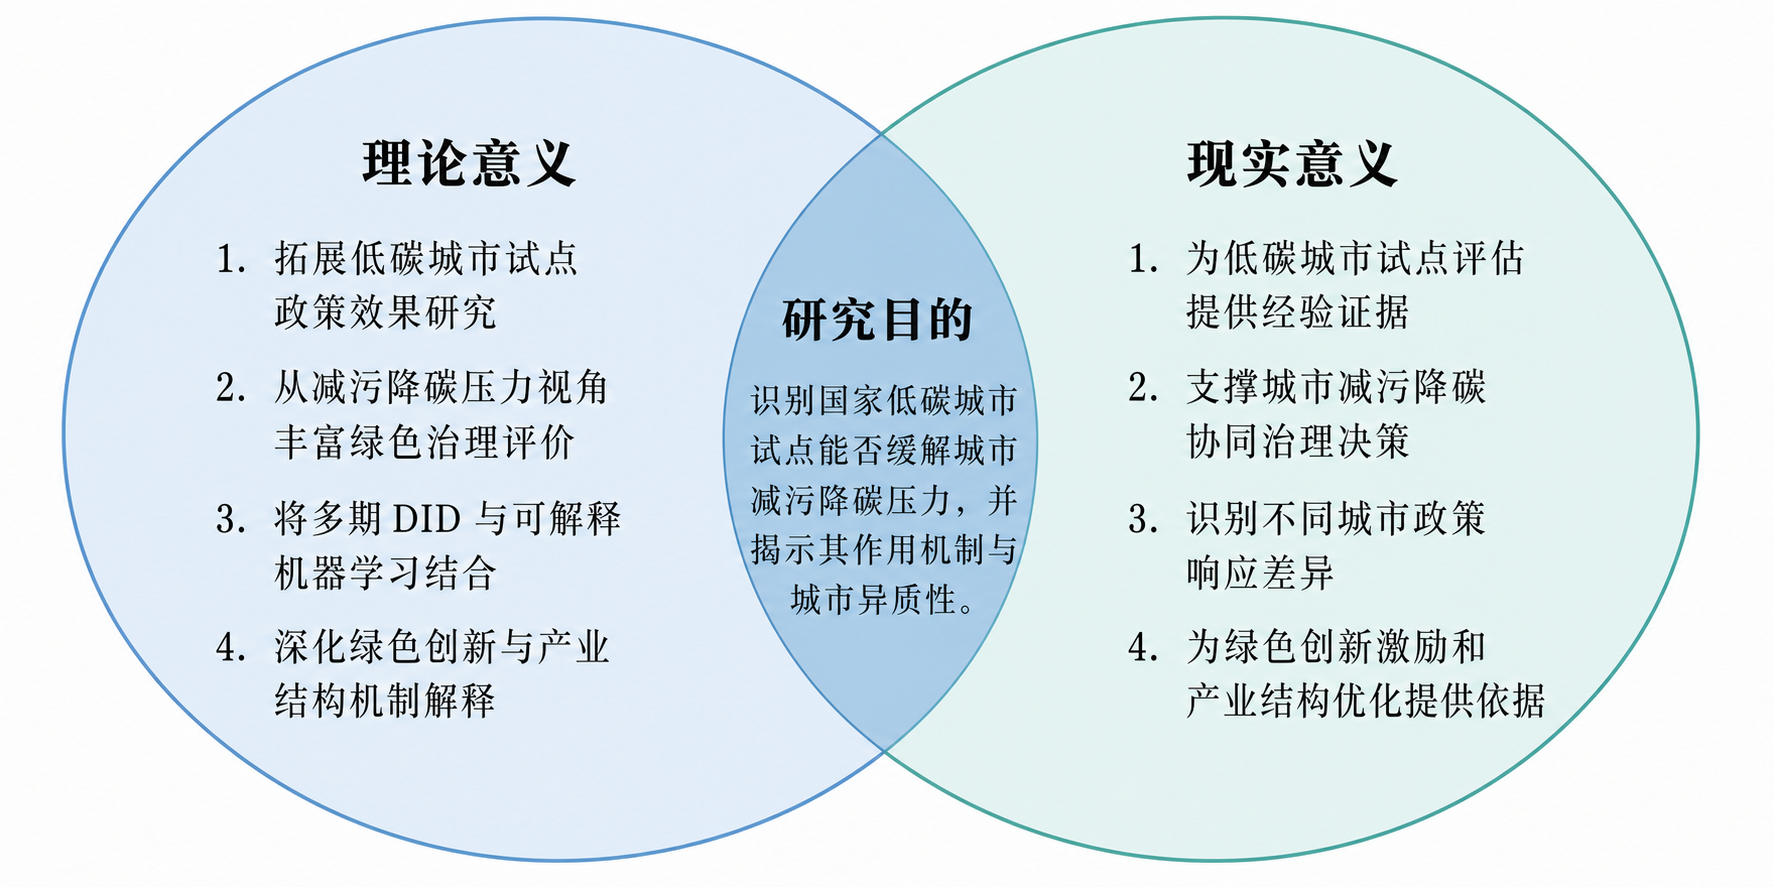
\includegraphics[width=\textwidth]{assets/figures/研究目的.png}
    \caption{研究目的与意义}
    \label{fig:research_purpose}
\end{figure}

本文聚焦国家低碳城市试点能否缓解城市减污降碳压力，并进一步分析其作用机制和异质性。本文的边际贡献主要体现在三个方面：第一，基于波特假说\footnote{波特假说认为，适当设计的环境规制能够激励企业开展技术创新，从而在改善环境绩效的同时提升资源配置效率和竞争力。}，本文从碳排放和污染排放两个维度构建减污降碳压力指数，用以评估低碳城市试点政策效果。第二，本文在识别低碳城市试点平均政策效应的基础上，进一步考察绿色创新的中介效应和产业结构的调节效应。第三，本文引入随机森林、XGBoost和TreeSHAP方法，在传统DID识别平均处理效应的基础上，进一步刻画个体城市在减污降碳压力和政策响应上的差异。

本文技术路径如图~\ref{fig:research_flow}所示。

\begin{figure}[H]
    \centering
    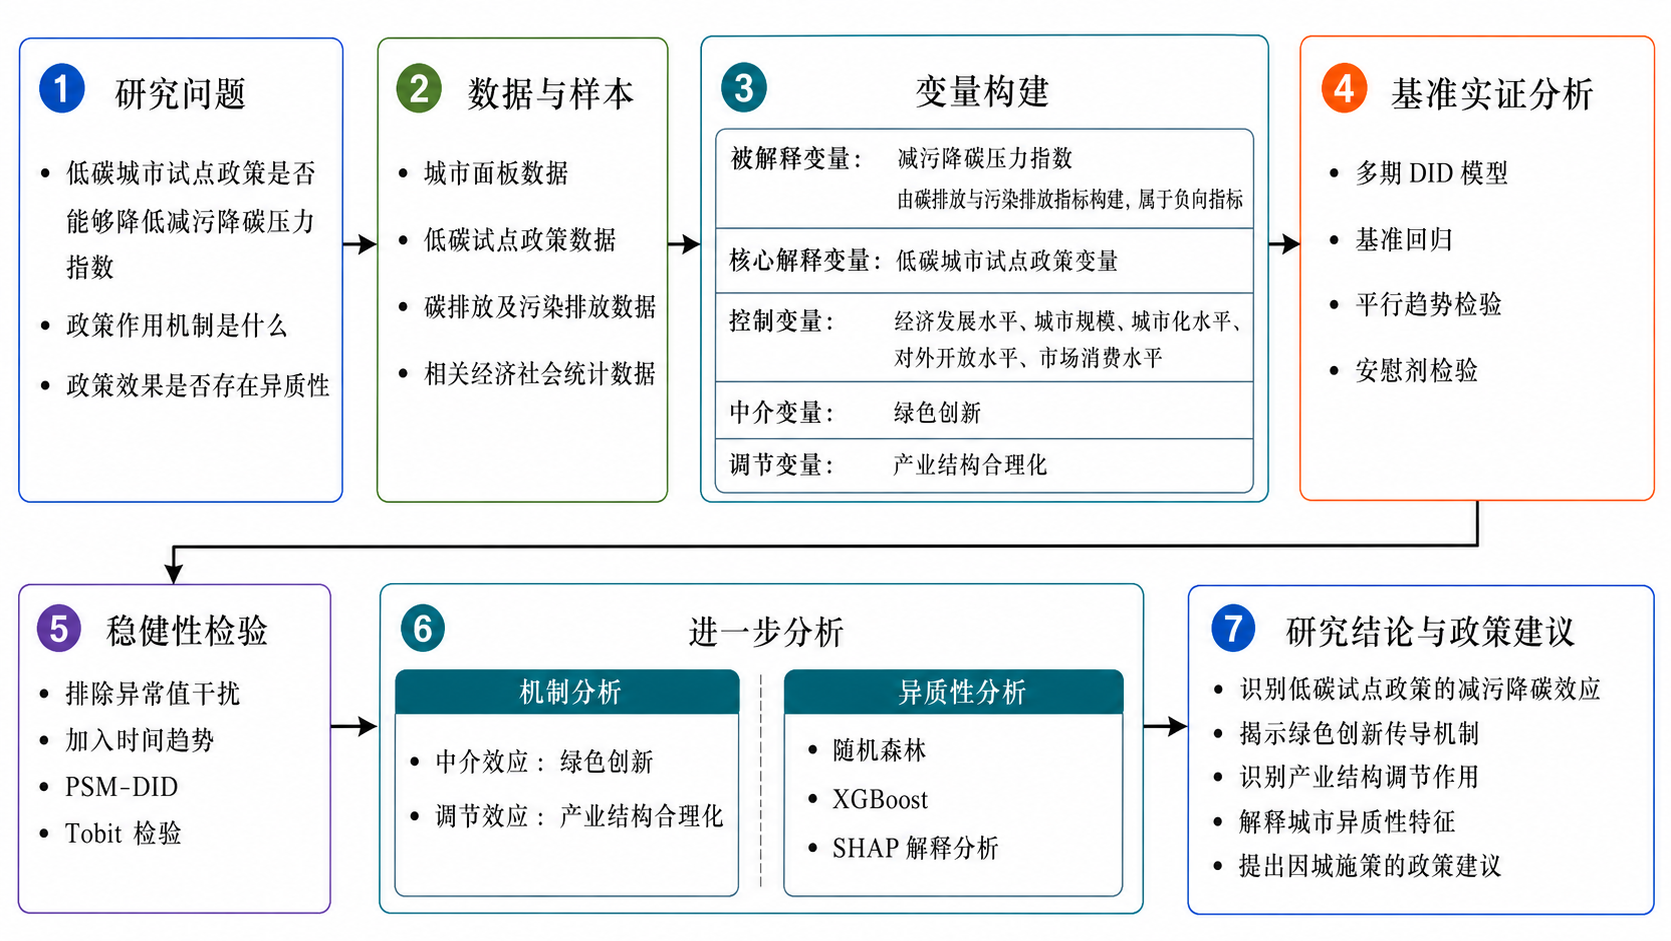
\includegraphics[width=\textwidth]{assets/figures/总流程图.png}
    \caption{技术路径图}
    \label{fig:research_flow}
\end{figure}

\section{文献综述}

\subsection{低碳城市试点政策效果}

关于低碳城市试点政策效果，现有研究大体围绕环境治理绩效、绿色发展绩效和城市转型效应三个方面展开。相关研究普遍发现，低碳城市试点在碳排放控制、污染治理和绿色效率提升方面具有一定效果，但其作用强度会因城市发展阶段、产业基础和治理能力不同而存在差异。邢华和李向阳（2024）以低碳城市试点为准自然实验，发现低碳城市试点能够在降低城市碳排放的同时减少环境污染，并具有一定治理效应；成喜玲和胡照远（2025）进一步从污碳减排角度考察低碳城市试点的政策效果；黄寰等（2023）则关注低碳城市试点的碳减排效应及其结构性作用。总体而言，现有低碳城市试点研究主要关注碳排放下降、污染治理改善和绿色发展绩效提升，但对减污降碳压力这一结果维度关注不足。

\subsection{减污降碳效应}

减污与降碳在排放来源和治理路径上具有较强关联，因此二者的耦合关系成为绿色低碳研究的重要议题。围绕减污降碳效应测度，已有研究采用耦合协调度模型、交乘指标、综合指数和效率评价模型等方式，刻画碳排放与污染排放之间的关联程度。罗良文和雷朱家华（2024）从碳市场政策角度考察减污降碳协同效应，强调需要同时识别碳排放和污染排放变化；张雪纯等（2024）基于碳排放交易制度讨论政策的减污降碳效应；刘明亮等（2024）从城市群视角分析减污降碳协同效率的时空演化特征。已有研究已形成较丰富的指标测度方法和政策评价体系，虽然关注了减污与降碳之间的耦合关系，但对城市减污降碳压力状态及其政策缓释作用关注不足。

\subsection{低碳城市试点机制与异质性}

低碳城市试点并非单一减排政策，而是包含环境规制、技术创新、产业调整和治理能力提升等内容的综合性政策安排。围绕政策作用机制，邢华和李向阳（2024）从规模效应、结构效应和技术效应解释低碳城市试点的治理作用；黄寰等（2023）指出产业结构调整是低碳城市试点发挥碳减排效应的重要路径；孙慧等（2025）对用能权交易制度与低碳城市双试点效应的讨论也表明，不同政策组合和城市条件会影响治理效果。相关研究为分析绿色创新中介效应和产业结构调节效应提供了基础，但对城市个体层面的差异解释仍相对不足。

\subsection{现有研究特点与不足}

综合来看，现有研究仍有进一步拓展空间。首先，现有研究多关注低碳城市试点能否产生减排、治污或效率提升效应，对其影响减污降碳压力的内在机制讨论仍有不足，尤其是绿色创新和产业结构在政策效果形成中的作用仍需进一步检验。其次，既有双重差分法主要识别平均处理效应，能够回答政策总体上是否有效，但难以从个体城市层面解释不同城市政策响应和减污降碳压力变化的差异。最后，现有研究多依赖单一模型设定，对不同模型设定下结果稳定性以及城市特征之间复杂交互关系的讨论仍显不足。因此，本文从减污降碳压力缓解问题出发，结合多期 DID、中介效应和调节效应的机制检验以及可解释机器学习方法，分析低碳城市试点的政策效果及城市个体差异。


\section{研究假设}

已有研究表明，低碳城市试点能够通过目标约束、能源结构调整和环境治理强化影响城市排放表现。邢华和李向阳（2024）发现，低碳城市试点能够在降低城市碳排放的同时减少环境污染；成喜玲和胡照远（2025）从污碳减排角度验证了试点政策的治理效应；黄寰等（2023）指出产业结构调整是试点政策发挥碳减排效应的重要路径。由此可见，低碳城市试点能够约束高耗能、高排放活动，同时作用于碳排放与污染排放，进而降低城市减污降碳压力。由此提出假设H1：

\noindent\textbf{\heiti H1：低碳城市试点政策能够显著降低城市减污降碳压力。}

绿色创新是低碳政策转化为环境绩效的重要渠道。邢华和李向阳（2024）从技术效应角度解释低碳城市试点的治理作用；张梦雨和马晓钰（2026）指出，新型基础设施和绿色技术创新有助于减污降碳效应的形成；郝浩宇等（2025）强调企业绿色技术创新对城市低碳绩效的重要影响。低碳城市试点能够通过目标约束、政策激励和环境规制强化，提升绿色创新激励，引导绿色技术研发与清洁生产技术应用，进而降低城市减污降碳压力。由此提出假设H2：

\noindent\textbf{\heiti H2：绿色创新在低碳城市试点政策降低城市减污降碳压力的过程中，发挥中介效应。}

产业结构会影响城市能源消费强度、污染排放基础和低碳政策转化效率。干春晖等（2011）从产业结构合理化角度刻画产业结构变迁，黄寰等（2023）指出产业结构调整是试点政策发挥减排作用的重要路径，孙慧等（2025）表明城市条件差异会影响降碳减污治理效果。产业结构越合理，资源配置效率越高，政策实施阻力和治理成本越低；反之，产业结构偏离均衡状态越明显，要素错配越严重，高耗能、高排放部门锁定效应越强，政策降低减污降碳压力的效果越弱。鉴于TL指数数值越大表示产业结构越偏离均衡，本文重点考察产业结构合理化变量在政策效应中的负向调节效应。由此提出假设H3：

\noindent\textbf{\heiti H3：产业结构合理化变量在低碳城市试点政策降低减污降碳压力过程中，发挥负向调节效应。}
\section{研究设计}

\subsection{数据来源与样本说明}

本文以2006—2021年中国277个地级及以上城市为研究样本。三批低碳城市试点名单分别来源于国家发展改革委发布的《关于开展低碳省区和低碳城市试点工作的通知》《关于开展第二批国家低碳省区和低碳城市试点工作的通知》和《关于开展第三批国家低碳城市试点工作的通知》。二氧化碳排放数据来源于 Figshare 平台公开发布的数据集《Dataset of City-level CO$_2$ emissions in China during 1992--2023》，绿色专利相关数据来源于国家知识产权局，其余数据主要来自 CSMAR 数据库和《中国城市统计年鉴》。

在样本整理过程中，本文对不同来源数据进行城市名称匹配和年份对齐，并统一变量的计量单位。对于连续型缺失指标，本文采用线性插值法进行补齐；对于关键变量长期缺失或明显异常的观测值，本文在数据清洗阶段予以识别和剔除，并对连续变量按1\%进行缩尾处理。经上述数据处理后，本文最终得到4432个有效样本，为后续实证分析提供数据基础。

\subsection{变量定义}

\subsubsection{被解释变量}

本文的被解释变量为减污降碳压力指数（$Pressure$）。借鉴邢华和李向阳（2024）关于减污降碳效应的测度思路，本文从碳排放维度和污染排放维度共同构建该指数，其中 $\ln CO_2$ 用于刻画城市碳排放压力，工业SO$_2$排放量、工业烟粉尘排放量和工业废水排放量用于刻画城市污染排放压力。本文采用 CRITIC 客观赋权法构建城市层面的减污降碳压力指数，基础指标及 CRITIC 权重如表~\ref{tab:critic_weight} 所示。

\begin{table}[H]
    \centering
    \caption{基础指标及 CRITIC 权重}
    \label{tab:critic_weight}
    \begin{threeparttable}
    \tablefont
    \renewcommand{\arraystretch}{1.2}
    \setlength{\tabcolsep}{2.5pt}
    \begin{tabular}{C{2.3cm}|C{2.3cm}|C{3.4cm}|C{1.4cm}|C{1.4cm}}
        \hline
        综合指标 & 一级指标 & 二级指标 & 指标属性 & 权重 \\
        \hline
        \multirow{4}{2.3cm}{\centering 减污降碳压力指数} & 碳排放水平 & $\ln CO_2$ & $+$ & 0.4570 \\
        \cline{2-5}
        & \multirow{3}{2.3cm}{\centering 污染排放水平} & 工业SO$_2$排放量 & $+$ & 0.2045 \\
        \cline{3-5}
        & & 工业烟尘排放量 & $+$ & 0.0770 \\
        \cline{3-5}
        & & 工业废水排放量 & $+$ & 0.2615 \\
        \hline
    \end{tabular}
    \end{threeparttable}
\end{table}

具体而言，设 $x_{ijt}$ 表示城市 $i$ 在年份 $t$ 的第 $j$ 项压力指标，本文首先对各指标进行 Min-Max 标准化处理，如公式（1）所示。
\begin{equation}
z_{ijt}=\frac{x_{ijt}-\min(x_j)}{\max(x_j)-\min(x_j)}
\end{equation}

在此基础上，以指标的标准差和指标间冲突性共同刻画其信息量，并计算 CRITIC 权重，如公式（2）所示。
\begin{equation}
C_j=\sigma_j \sum_{k=1}^{m}(1-r_{jk}), \qquad
w_j=\frac{C_j}{\sum_{j=1}^{m} C_j}
\end{equation}

最终得到城市层面的减污降碳压力指数，如公式（3）所示。
\begin{equation}
Pressure_{it}=\sum_{j=1}^{m} w_j z_{ijt}
\end{equation}

\subsubsection{核心解释变量}

本文的核心解释变量为低碳城市试点政策变量，记为 $DID_{it}$。本文先定义试点城市虚拟变量 $Treat_i$ 与政策实施前后的时间虚拟变量 $Post_t$，再构造双重差分变量。
\begin{equation}
DID_{it}=Treat_i\times Post_t
\end{equation}

其中，若城市 $i$ 属于国家低碳城市试点城市，则 $Treat_i=1$，否则 $Treat_i=0$；$G_i$ 表示城市 $i$ 的政策启动年份，若 $t\geq G_i$，则 $Post_t=1$，否则 $Post_t=0$。具体赋值上，第一批试点自2010年起进入处理期，第二批试点因名单于2012年11月公布较晚，本文自2013年起进入处理期，第三批试点自2017年起进入处理期，其余城市-年份观测值均赋值为0，据此构建多期 DID 政策变量。该设定既保持了政策识别与制度实施时点的一致性，也尽可能避免因名单公布时间过晚造成的处理期误判。

\begin{figure}[H]
    \centering
    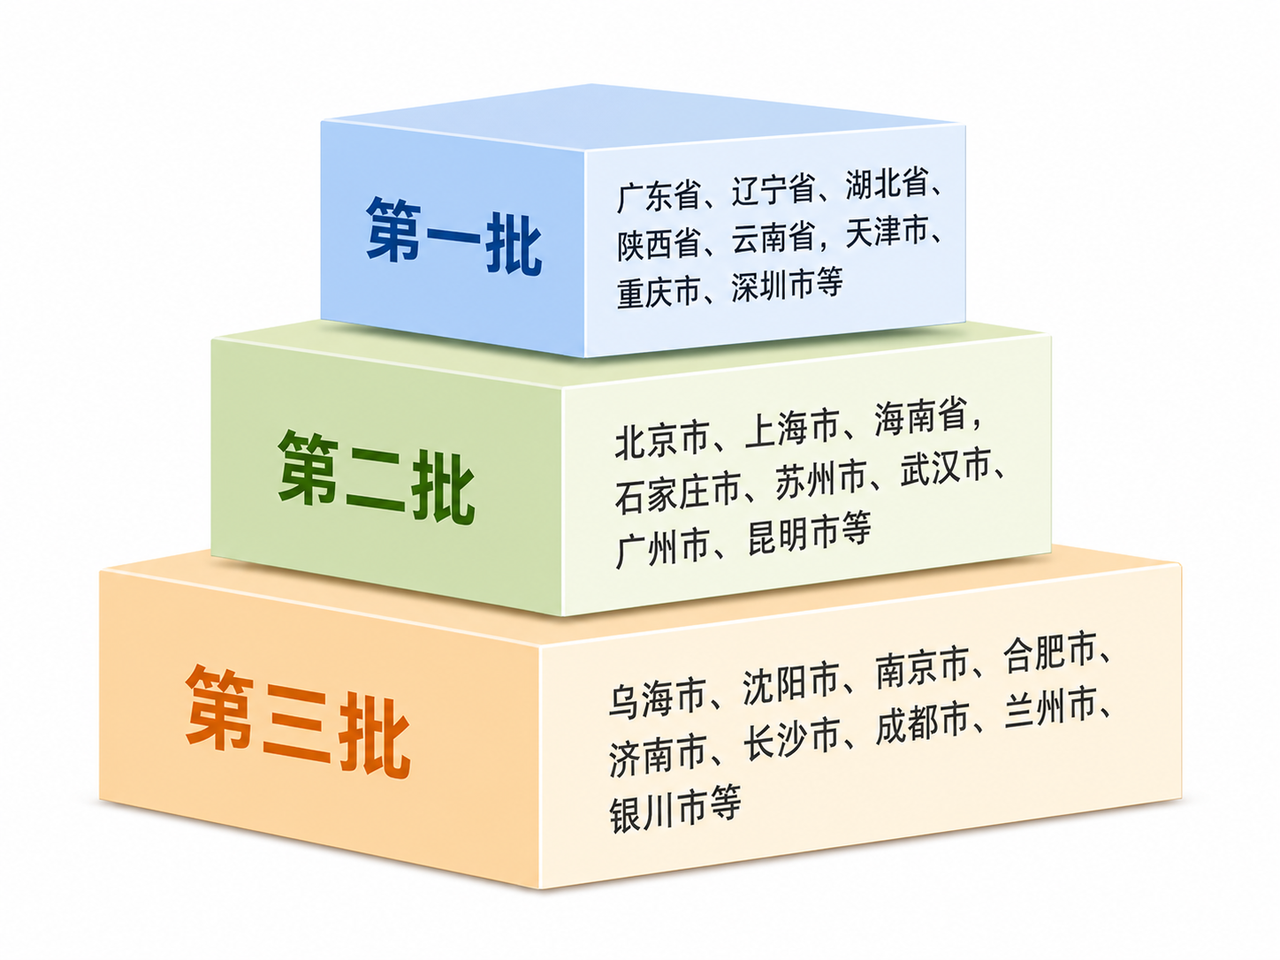
\includegraphics[width=0.62\textwidth]{assets/figures/政策试点城市图.png}
    \caption{低碳城市试点示意图}
    \label{fig:pilot_batches}
\end{figure}

\subsubsection{控制变量}

为尽可能控制其他影响城市减污降碳压力指数的因素，减少遗漏变量偏误，本文综合借鉴邢华和李向阳（2024）以及罗良文和雷朱家华（2024）相关研究的做法，选取经济发展水平（$lnpgdp$）、城市规模（$lnpop$）、城市化水平（$urban$）、对外开放水平（$fdi$）和市场消费水平（$retail$）作为控制变量。其中，经济发展水平以人均 GDP 取对数衡量，城市规模以总人口取对数衡量，城市化水平以城镇人口占总人口比重衡量，对外开放水平以外商实际投资额占 GDP 比重衡量，市场消费水平以社会消费品零售总额占 GDP 比重衡量。

\subsubsection{中介变量}

为进一步检验低碳城市试点政策影响城市减污降碳压力的作用机制，本文选取绿色创新（greeninnov）作为中介变量。已有研究常用绿色专利刻画城市绿色创新能力，本文借鉴郝浩宇等（2025）关于绿色创新测度的研究思路，并结合研究需要进行调整。具体而言，本文以各城市辖区内企业的发明型绿色专利数和授权型绿色专利数之和来衡量该城市的绿色创新水平。

\subsubsection{调节变量}

为进一步考察产业结构特征对低碳城市试点政策减污降碳压力缓解效果的调节效应，本文选取产业结构合理化（$TL$）作为调节变量。参考干春晖等（2011）关于产业结构变迁的测度方法，并借鉴罗良文和雷朱家华（2024）的相关表述，本文采用 Theil 指数衡量产业结构合理化水平，以反映产业间产出结构与就业结构的匹配程度。其计算方式如公式（5）所示。
\begin{equation}
TL_{it}=\sum_{m=1}^{3}\left(\frac{Y_{mit}}{Y_{it}}\right)\ln\left(\frac{Y_{mit}/Y_{it}}{L_{mit}/L_{it}}\right)
\end{equation}

其中，$Y_{mit}$ 表示城市 $i$ 在年份 $t$ 的第 $m$ 产业产出，$L_{mit}$ 表示第 $m$ 产业就业人数，$Y_{it}$ 和 $L_{it}$ 分别表示城市总产出与总就业人数。若 $TL_{it}\neq 0$，则表明产业结构偏离均衡状态，且数值越大，产业结构越不合理。

综合上述设定，本文主要变量如表~\ref{tab:variables} 所示。

\begin{table}[H]
    \centering
    \caption{主要变量说明}
    \label{tab:variables}
    \begin{threeparttable}
    \tablefont
    \renewcommand{\arraystretch}{1.45}
    \setlength{\extrarowheight}{2pt}
    \setlength{\tabcolsep}{1pt}
    \renewcommand{\tabularxcolumn}[1]{>{\raggedright\arraybackslash}m{#1}}
    \begin{tabularx}{\textwidth}{>{\centering\arraybackslash}m{2.45cm}>{\centering\arraybackslash}m{4.0cm}>{\centering\arraybackslash}m{2.2cm}>{\raggedright\arraybackslash}X}
        \toprule
        变量类别 & 中文名称 & 变量符号 & 变量说明 \\
        \midrule
        被解释变量 & 减污降碳压力指数 & $Pressure_{it}$ & 基于 $\ln CO_2$、工业SO$_2$排放量、工业烟粉尘排放量和工业废水排放量构建的 CRITIC 综合指数。 \\
        \midrule
        核心解释变量 & 低碳城市试点政策变量 & $DID_{it}$ & 由 $Treat_i$ 与 $Post_t$ 相乘得到，反映城市 $i$ 在年份 $t$ 的政策处理状态。 \\
        \midrule
        \multirow{5}{*}{控制变量} & 经济发展水平 & $lnpgdp_{it}$ & 人均 GDP 取对数。 \\
        & 城市规模 & $lnpop_{it}$ & 总人口取对数。 \\
        & 城市化水平 & $urban_{it}$ & 城镇人口占总人口比重。 \\
        & 对外开放水平 & $fdi_{it}$ & 外商实际投资额占 GDP 比重。 \\
        & 市场消费水平 & $retail_{it}$ & 社会消费品零售总额占 GDP 比重。 \\
        \midrule
        中介变量 & 绿色创新 & $greeninnov_{it}$ & 企业发明型和授权型绿色专利数之和。 \\
        \midrule
        调节变量 & 产业结构合理化 & $TL_{it}$ & Theil 指数，数值越大表示产业结构越偏离均衡状态。 \\
        \bottomrule
    \end{tabularx}
    \end{threeparttable}
\end{table}

\subsection{模型设定}

\subsubsection{基准回归}

为评估低碳城市试点政策对减污降碳压力的影响，本文基于城市-年份面板数据构建多期 DID 双向固定效应模型，具体设定如公式（6）所示。
\begin{equation}
Pressure_{it}=\alpha_0+\alpha_1 DID_{it}+\alpha_2 Treat_i+\alpha_3 Post_t+\boldsymbol{\gamma}'\mathbf{X}_{it}+\mu_i+\lambda_t+\varepsilon_{it}
\end{equation}

其中，$Pressure_{it}$ 为本文的被解释变量，即城市 $i$ 在年份 $t$ 的减污降碳压力指数；$DID_{it}$ 为本文的核心解释变量，即低碳城市试点政策变量；$\mathbf{X}_{it}$ 表示控制变量向量；$\boldsymbol{\gamma}$ 为其对应的待估系数向量；$\alpha_1$ 为本文重点关注的政策效应系数，预期显著为负，表示低碳城市试点政策能够缓解减污降碳压力；$\mu_i$ 为城市固定效应；$\lambda_t$ 为年份固定效应；$\varepsilon_{it}$ 为随机扰动项。

\subsubsection{平行趋势检验}

政策处理效应可信的重要前提之一是处理组与控制组在政策实施前满足平行趋势假设。为此，本文采用事件研究法对政策实施前后的效应进行识别，并同时检验政策作用的时序特征。平行趋势检验模型见公式（7）。
\begin{equation}
Pressure_{it}=\alpha+\sum_{k=-3,k\neq -1}^{4}\beta_k D_{i,t_0+k}+\boldsymbol{\delta}'\mathbf{X}_{it}+\mu_i+\lambda_t+\varepsilon_{it}
\end{equation}

其中，$D_{i,t_0+k}$ 为政策实施相对年份的系列虚拟变量，$t_0$ 表示城市 $i$ 正式进入低碳城市试点的真实年份，$k$ 为相对时间标识。借鉴已有研究惯例，本文将政策实施前一年（$k=-1$）作为基准期。$\beta_k$ 为模型核心估计参数，用于衡量政策实施第 $k$ 年处理组与控制组减污降碳压力指数的相对净差异。若政策实施前各期系数整体不显著，则说明样本基本满足平行趋势假设。

\subsubsection{安慰剂检验}

为排除样本随机性所导致的“伪显著”问题，本文采用基于虚拟处理组的安慰剂检验。具体而言，本文在全部样本中随机抽取与真实试点数量相同的城市作为“伪处理组”，并据此构造虚拟低碳城市试点变量。本文重复上述随机抽样过程 500 次并重新估计基准模型。若真实政策变量的估计系数明显偏离虚拟政策系数分布，则说明基准回归结果并非由随机因素驱动，从而进一步说明低碳城市试点政策效应具有有效性。

\subsubsection{中介效应}

为探究低碳城市试点政策影响减污降碳压力的具体传导路径，本文借鉴温忠麟等（2004）提出的中介效应检验思路，采用三步回归法构建中介效应模型，对绿色创新的中介机制进行检验。
\begin{equation}
Pressure_{it}=\alpha_0+\alpha_1 DID_{it}+\alpha_2 Treat_i+\alpha_3 Post_t+\boldsymbol{\gamma}'\mathbf{X}_{it}+\mu_i+\lambda_t+\varepsilon_{it}
\end{equation}
\begin{equation}
greeninnov_{it}=\rho_0+\rho_1 DID_{it}+\rho_2 Treat_i+\rho_3 Post_t+\boldsymbol{\gamma}'\mathbf{X}_{it}+\mu_i+\lambda_t+\varepsilon_{it}
\end{equation}
\begin{equation}
\begin{split}
Pressure_{it}={}&\pi_0+\pi_1 DID_{it}+\pi_2 greeninnov_{it}+\pi_3 Treat_i \\
&+\pi_4 Post_t+\boldsymbol{\gamma}'\mathbf{X}_{it}
+\mu_i+\lambda_t+\varepsilon_{it}
\end{split}
\end{equation}

其中，$greeninnov_{it}$ 为中介变量，即城市绿色创新水平。$\rho_1$ 反映低碳城市试点政策对绿色创新的影响，$\pi_2$ 反映绿色创新对减污降碳压力指数的影响。若 $\rho_1$ 与 $\pi_2$ 同时显著，且纳入中介变量后核心政策系数的绝对值发生变化，则说明低碳城市试点可能通过绿色创新路径影响城市减污降碳压力指数；间接效应可表示为 $\rho_1\times\pi_2$。进一步地，本文采用 Bootstrap 方法对间接效应进行检验，通过重复抽样 500 次构造间接效应的经验分布，并计算其置信区间。若 Bootstrap 置信区间不包含0，则说明中介效应显著存在。

\subsubsection{调节效应}

考虑到低碳城市试点的政策效果可能因城市产业结构合理化水平不同而呈现差异性，本文在基准模型中引入调节变量及其与政策变量的交互项，构建调节效应模型。
\begin{equation}
\begin{split}
Pressure_{it}={}&\theta_0+\theta_1(DID_{it}\times TL_{it})+\theta_2 DID_{it}+\theta_3 TL_{it} \\
&+\boldsymbol{\gamma}'\mathbf{X}_{it}+\mu_i+\lambda_t+\varepsilon_{it}
\end{split}
\end{equation}

其中，$TL_{it}$ 表示产业结构合理化变量，数值越大表示产业结构偏离均衡状态越明显；$\theta_1$ 为政策变量与产业结构合理化变量的交互项系数，用于考察产业结构差异是否会影响低碳城市试点政策的减污降碳压力缓解效果。若交互项显著，则说明产业结构合理化变量在低碳城市试点政策效应中发挥调节效应。结合 $TL$ 指标方向，本文重点关注产业结构偏离均衡状态是否会削弱政策效果。

\subsection{机器学习与可解释性方法}

\subsubsection{随机森林}

随机森林（Random Forest）是集成学习中 Bagging 思想的典型代表。该方法通过 Bootstrap 重抽样构建多棵回归树，提高模型的稳健性与抗过拟合能力。对于本文的连续型目标变量，其预测值可表示为：
\begin{equation}
\hat{y}_i^{RF}=\frac{1}{B}\sum_{b=1}^{B}f_b(x_i)
\end{equation}

其中，$B$ 为决策树数量，$f_b(x_i)$ 为第 $b$ 棵回归树对样本 $x_i$ 的预测结果。

\subsubsection{XGBoost}

极端梯度提升树（XGBoost）是基于 Boosting 框架的集成学习算法。对任一给定样本 $x_i$，其预测值可表示为：
\begin{equation}
\hat{y}_i=\sum_{k=1}^{K}f_k(x_i), \qquad f_k \in \mathcal{F}
\end{equation}

为学习最优函数 $f_k$，XGBoost 在第 $t$ 轮迭代中的目标函数可写为：
\begin{equation}
\mathcal{L}^{(t)}=\sum_{i=1}^{n}l\left(y_i,\hat{y}_i^{(t-1)}+f_t(x_i)\right)+\Omega(f_t)
\end{equation}

其中，$l(\cdot)$ 为损失函数，$\Omega(f_t)=\gamma T+\frac{1}{2}\lambda ||w||^2$ 为正则化项，$T$ 表示叶子节点数，$w$ 表示叶子节点权重。进一步地，对目标函数作二阶泰勒展开，可得：
\begin{equation}
\mathcal{L}^{(t)} \approx \sum_{i=1}^{n}\left[g_i f_t(x_i)+\frac{1}{2}h_i f_t^2(x_i)\right]+\Omega(f_t)+C
\end{equation}

其中，$g_i$ 和 $h_i$ 分别表示损失函数关于上一轮预测值的一阶偏导数和二阶偏导数，$C$ 为与本轮优化无关的常数项。

\subsubsection{参数设置与模型评价指标}

为提高模型性能，本文采用 5 折交叉验证在训练集上进行参数调优，并以 RMSE 等指标评价模型性能，最终参数见表~\ref{tab:ml_params}。

\begin{table}[H]
    \centering
    \caption{随机森林与 XGBoost 参数设置}
    \label{tab:ml_params}
    \renewcommand{\arraystretch}{1.18}
    \begin{threeparttable}
    \tablefont
    \setlength{\tabcolsep}{4pt}
    \begin{tabularx}{\textwidth}{C{1.9cm}C{3.3cm}C{4.1cm}C{1.8cm}}
        \toprule
        模型 & 参数 & 代码表示 & 最优取值 \\
        \midrule
        \multirow{3}{*}{\textbf{随机森林}}
        & 树数 & \texttt{n\_estimators} & 600 \\
        & 特征比例 & \texttt{max\_features} & 1.0 \\
        & 叶节点最小样本数 & \texttt{min\_samples\_leaf} & 1 \\
        \addlinespace[2pt]
        \midrule
        \addlinespace[2pt]
        \multirow{5}{*}{\textbf{XGBoost}}
        & 树数 & \texttt{n\_estimators} & 600 \\
        & 最大深度 & \texttt{max\_depth} & 4 \\
        & 学习率 & \texttt{learning\_rate} & 0.05 \\
        & 行采样比例 & \texttt{subsample} & 0.8 \\
        & 列采样比例 & \texttt{colsample\_bytree} & 1.0 \\
        \bottomrule
    \end{tabularx}
    \begin{tablenotes}[flushleft]
        \tablenotefont
        \item 注：表中报告网格搜索后的最优参数组合。
    \end{tablenotes}
    \end{threeparttable}
\end{table}

\subsubsection{TreeSHAP 可解释性框架}

尽管随机森林和 XGBoost 等集成学习算法具有较强的拟合能力，但其模型结构较为复杂，且具有典型的“黑箱”特征。为此，本文引入 TreeSHAP（Tree Shapley Additive Explanations）归因框架对最优机器学习模型进行事后解释。对于给定样本 $x$，特征 $j$ 的 TreeSHAP 值可表示为：
\begin{equation}
\phi_j=\sum_{S\subseteq N\setminus \{j\}}\frac{|S|!(M-|S|-1)!}{M!}\left[f_x(S\cup \{j\})-f_x(S)\right]
\end{equation}

其中，$N$ 为全部特征集合，$S$ 为不包含特征 $j$ 的任意特征子集，$M$ 为特征总数；$f_x(S)$ 表示模型在特征子集 $S$ 上的预测期望。

\subsubsection{算法流程}

本文先利用随机森林和 XGBoost 进行横向对比，识别影响城市减污降碳压力的关键特征，再引入 TreeSHAP 解释框架对最优模型进行纵向深化，从平均层面推进至个体层面的异质性分析。

\begin{center}
\begin{minipage}{0.96\textwidth}
\hrule
\vspace{0.12\baselineskip}
\noindent\textbf{Algorithm 1} RF--XGBoost--TreeSHAP 方法流程
\vspace{0.12\baselineskip}
\hrule
\vspace{0.16\baselineskip}
\small
\renewcommand{\arraystretch}{1.05}
\begin{tabularx}{\textwidth}{@{}l@{ }X@{}}
\textbf{Require:} & 城市面板样本 $(\mathcal{X}_{it},Pressure_{it})$；随机森林与 XGBoost 参数 $B,K,\eta$； \\
\textbf{Ensure:} & 最优树模型 $F^\ast$；性能指标、TreeSHAP 可解释性等； \\
\end{tabularx}
\vspace{0.04\baselineskip}
\begin{tabularx}{\textwidth}{@{}r@{\ }X@{}}
1: & 对城市-年份样本进行缺失值处理和标准化整理；划分训练集与测试集； \\
2: & 采用 Bootstrap 抽样训练随机森林；集成 $B$ 棵回归树并获得预测结果； \\
3: & 以平方误差损失训练 XGBoost；在学习率 $\eta$ 下迭代 $K$ 轮并更新树模型； \\
4: & 基于测试集 RMSE、MAE、$R^2$ 比较两类模型；确定模型性能更优的 $F^\ast$； \\
5: & 对 $F^\ast$ 计算 TreeSHAP 值 $\phi_j$；刻画各特征对模型输出的边际贡献； \\
\multicolumn{2}{@{}l@{}}{\textbf{Return:} 模型性能指标、特征重要性排序、TreeSHAP 摘要图与交互图。} \\
\end{tabularx}
\vspace{0.12\baselineskip}
\hrule
\end{minipage}
\end{center}

\section{实证结果与分析}

\subsection{描述性统计}

表~\ref{tab:desc}报告了主要变量的描述性统计。核心被解释变量 $Pressure$ 的均值为0.2572，标准差为0.0894，样本极差较大，表明样本城市在污染排放与碳排放压力方面差异明显。核心解释变量 $DID$ 的均值为0.1081，说明样本中处于低碳城市试点政策处理状态的城市-年份观测占比为10.81\%。进一步地，本文计算主要解释变量的方差膨胀因子，平均 VIF 为1.45，表明解释变量之间不存在严重多重共线性问题。主要变量描述性统计结果与现有研究基本一致，保证研究结果可比性。

\begin{table}[H]
    \centering
    \caption{描述性统计}
    \label{tab:desc}
    \tablefont
    \renewcommand{\arraystretch}{1.12}
    \begin{threeparttable}
    \setlength{\tabcolsep}{2pt}
    \begin{tabularx}{\textwidth}{C{2.3cm}C{2.0cm}*{5}{>{\centering\arraybackslash}X}}
        \toprule
        变量类别 & 变量名称 & 样本量 N & 均值 & 标准差 & 最小值 & 最大值 \\
        \midrule
        被解释变量 & Pressure & 4432 & 0.2572 & 0.0894 & 0.0166 & 0.7344 \\
        \midrule
        核心解释变量 & DID & 4432 & 0.1081 & 0.3105 & 0 & 1 \\
        \midrule
        \multirow{5}{*}{控制变量} & lnpgdp & 4432 & 10.2991 & 0.8060 & 7.9772 & 12.9575 \\
         & lnpop & 4432 & 5.8698 & 0.6976 & 2.9463 & 8.1363 \\
         & urban & 4432 & 0.4381 & 0.2006 & 0.0128 & 1 \\
         & fdi & 4432 & 0.0034 & 0.0043 & 0 & 0.0702 \\
         & retail & 4432 & 0.4530 & 0.1508 & 0 & 1.4033 \\
        \midrule
        中介变量 & greeninnov & 4432 & 530.0749 & 1780.5559 & 0 & 32661 \\
        \midrule
        调节变量 & TL & 4160 & 0.2659 & 0.2073 & -0.1409 & 1.7205 \\
        \bottomrule
    \end{tabularx}
    \begin{tablenotes}[flushleft]
        \tablenotefont
        \item 注：样本总量为4432，城市数量为277，年份范围为2006--2021年。产业结构合理化变量 $TL$ 的样本年份范围同样为2006--2021年，但因16个城市在2006--2021年的就业结构原始指标全部缺失，故有效样本量为4160。
    \end{tablenotes}
    \end{threeparttable}
\end{table}

\subsection{基准回归}

表~\ref{tab:baseline}报告了国家低碳城市试点对减污降碳压力指数影响的基准回归。列(1)仅控制城市固定效应和年份固定效应，列(2)至列(6)依次加入控制变量，以检验模型设定的稳健性。

\begin{table}[H]
    \centering
    \caption{基准回归}
    \label{tab:baseline}
    \begin{threeparttable}
    \renewcommand{\arraystretch}{1.08}
    \songti\fontsize{10pt}{12.5pt}\selectfont
    \setlength{\tabcolsep}{1.5pt}
    \begin{tabularx}{\textwidth}{L{2.45cm}*{6}{>{\centering\arraybackslash}X}}
        \toprule
        \multirow{2}{*}{\makebox[2.45cm][c]{变量符号}} & \multicolumn{6}{c}{Pressure} \\
        \cmidrule(lr){2-7}
         & (1) & (2) & (3) & (4) & (5) & (6) \\
        \midrule
        DID & \mbox{$-0.0145^{***}$} & \mbox{$-0.0143^{***}$} & \mbox{$-0.0144^{***}$} & \mbox{$-0.0150^{***}$} & \mbox{$-0.0150^{***}$} & \mbox{$-0.0152^{***}$} \\
          & (0.0042) & (0.0042) & (0.0041) & (0.0040) & (0.0040) & (0.0040) \\
        lnpgdp &  & 0.0407*** & 0.0466*** & 0.0634*** & 0.0637*** & 0.0626*** \\
          &  & (0.0097) & (0.0097) & (0.0142) & (0.0144) & (0.0144) \\
        urban &  &  & \mbox{$-0.0763^{***}$} & \mbox{$-0.0796^{***}$} & \mbox{$-0.0798^{***}$} & \mbox{$-0.0827^{***}$} \\
          &  &  & (0.0178) & (0.0175) & (0.0174) & (0.0170) \\
        lnpop &  &  &  & 0.0295** & 0.0300** & 0.0274* \\
          &  &  &  & (0.0141) & (0.0146) & (0.0147) \\
        fdi &  &  &  &  & \mbox{$-0.0541$} & \mbox{$-0.0644$} \\
          &  &  &  &  & (0.2459) & (0.2425) \\
        retail &  &  &  &  &  & 0.0165* \\
          &  &  &  &  &  & (0.0087) \\
        城市固定效应 & 是 & 是 & 是 & 是 & 是 & 是 \\
        年份固定效应 & 是 & 是 & 是 & 是 & 是 & 是 \\
        样本量 N & 4432 & 4432 & 4432 & 4432 & 4432 & 4432 \\
        调整后$R^2$ & 0.9300 & 0.9319 & 0.9336 & 0.9339 & 0.9339 & 0.9341 \\
        \bottomrule
    \end{tabularx}
    \begin{tablenotes}[flushleft]
        \tablenotefont
        \item 注：*、**、*** 分别表示在10\%、5\%、1\%水平上显著。括号内为按城市层级聚类的稳健标准误。下同。
    \end{tablenotes}
    \end{threeparttable}
\end{table}

表~\ref{tab:baseline}显示，随着控制变量逐步加入，低碳城市试点变量的估计系数始终显著为负。该结果表明，在控制一系列城市特征变量后，国家低碳城市试点政策仍能够显著缓解样本城市的综合减污降碳压力，假设H1得到验证。

从控制变量结果看，经济发展水平的系数显著为正，说明在样本期内经济活动强度提升仍可能伴随更高的减污降碳压力；城镇化水平系数显著为负，表明城市化进程可能通过基础设施完善、公共治理能力提升等途径缓解减污降碳压力；人口规模系数为正且在部分模型中显著，反映人口集聚可能增加资源消耗和环境治理难度。主要控制变量回归结果与现有文献基本一致。

\subsection{平行趋势检验}

图~\ref{fig:parallel}报告了平行趋势检验结果。政策实施前检验的 $p$ 值为0.1888，未能拒绝“政策实施前各期系数共同为零”的原假设，说明处理组与控制组在试点政策发生前不存在显著的系统性趋势差异，平行趋势假设成立。

\begin{figure}[H]
    \centering
    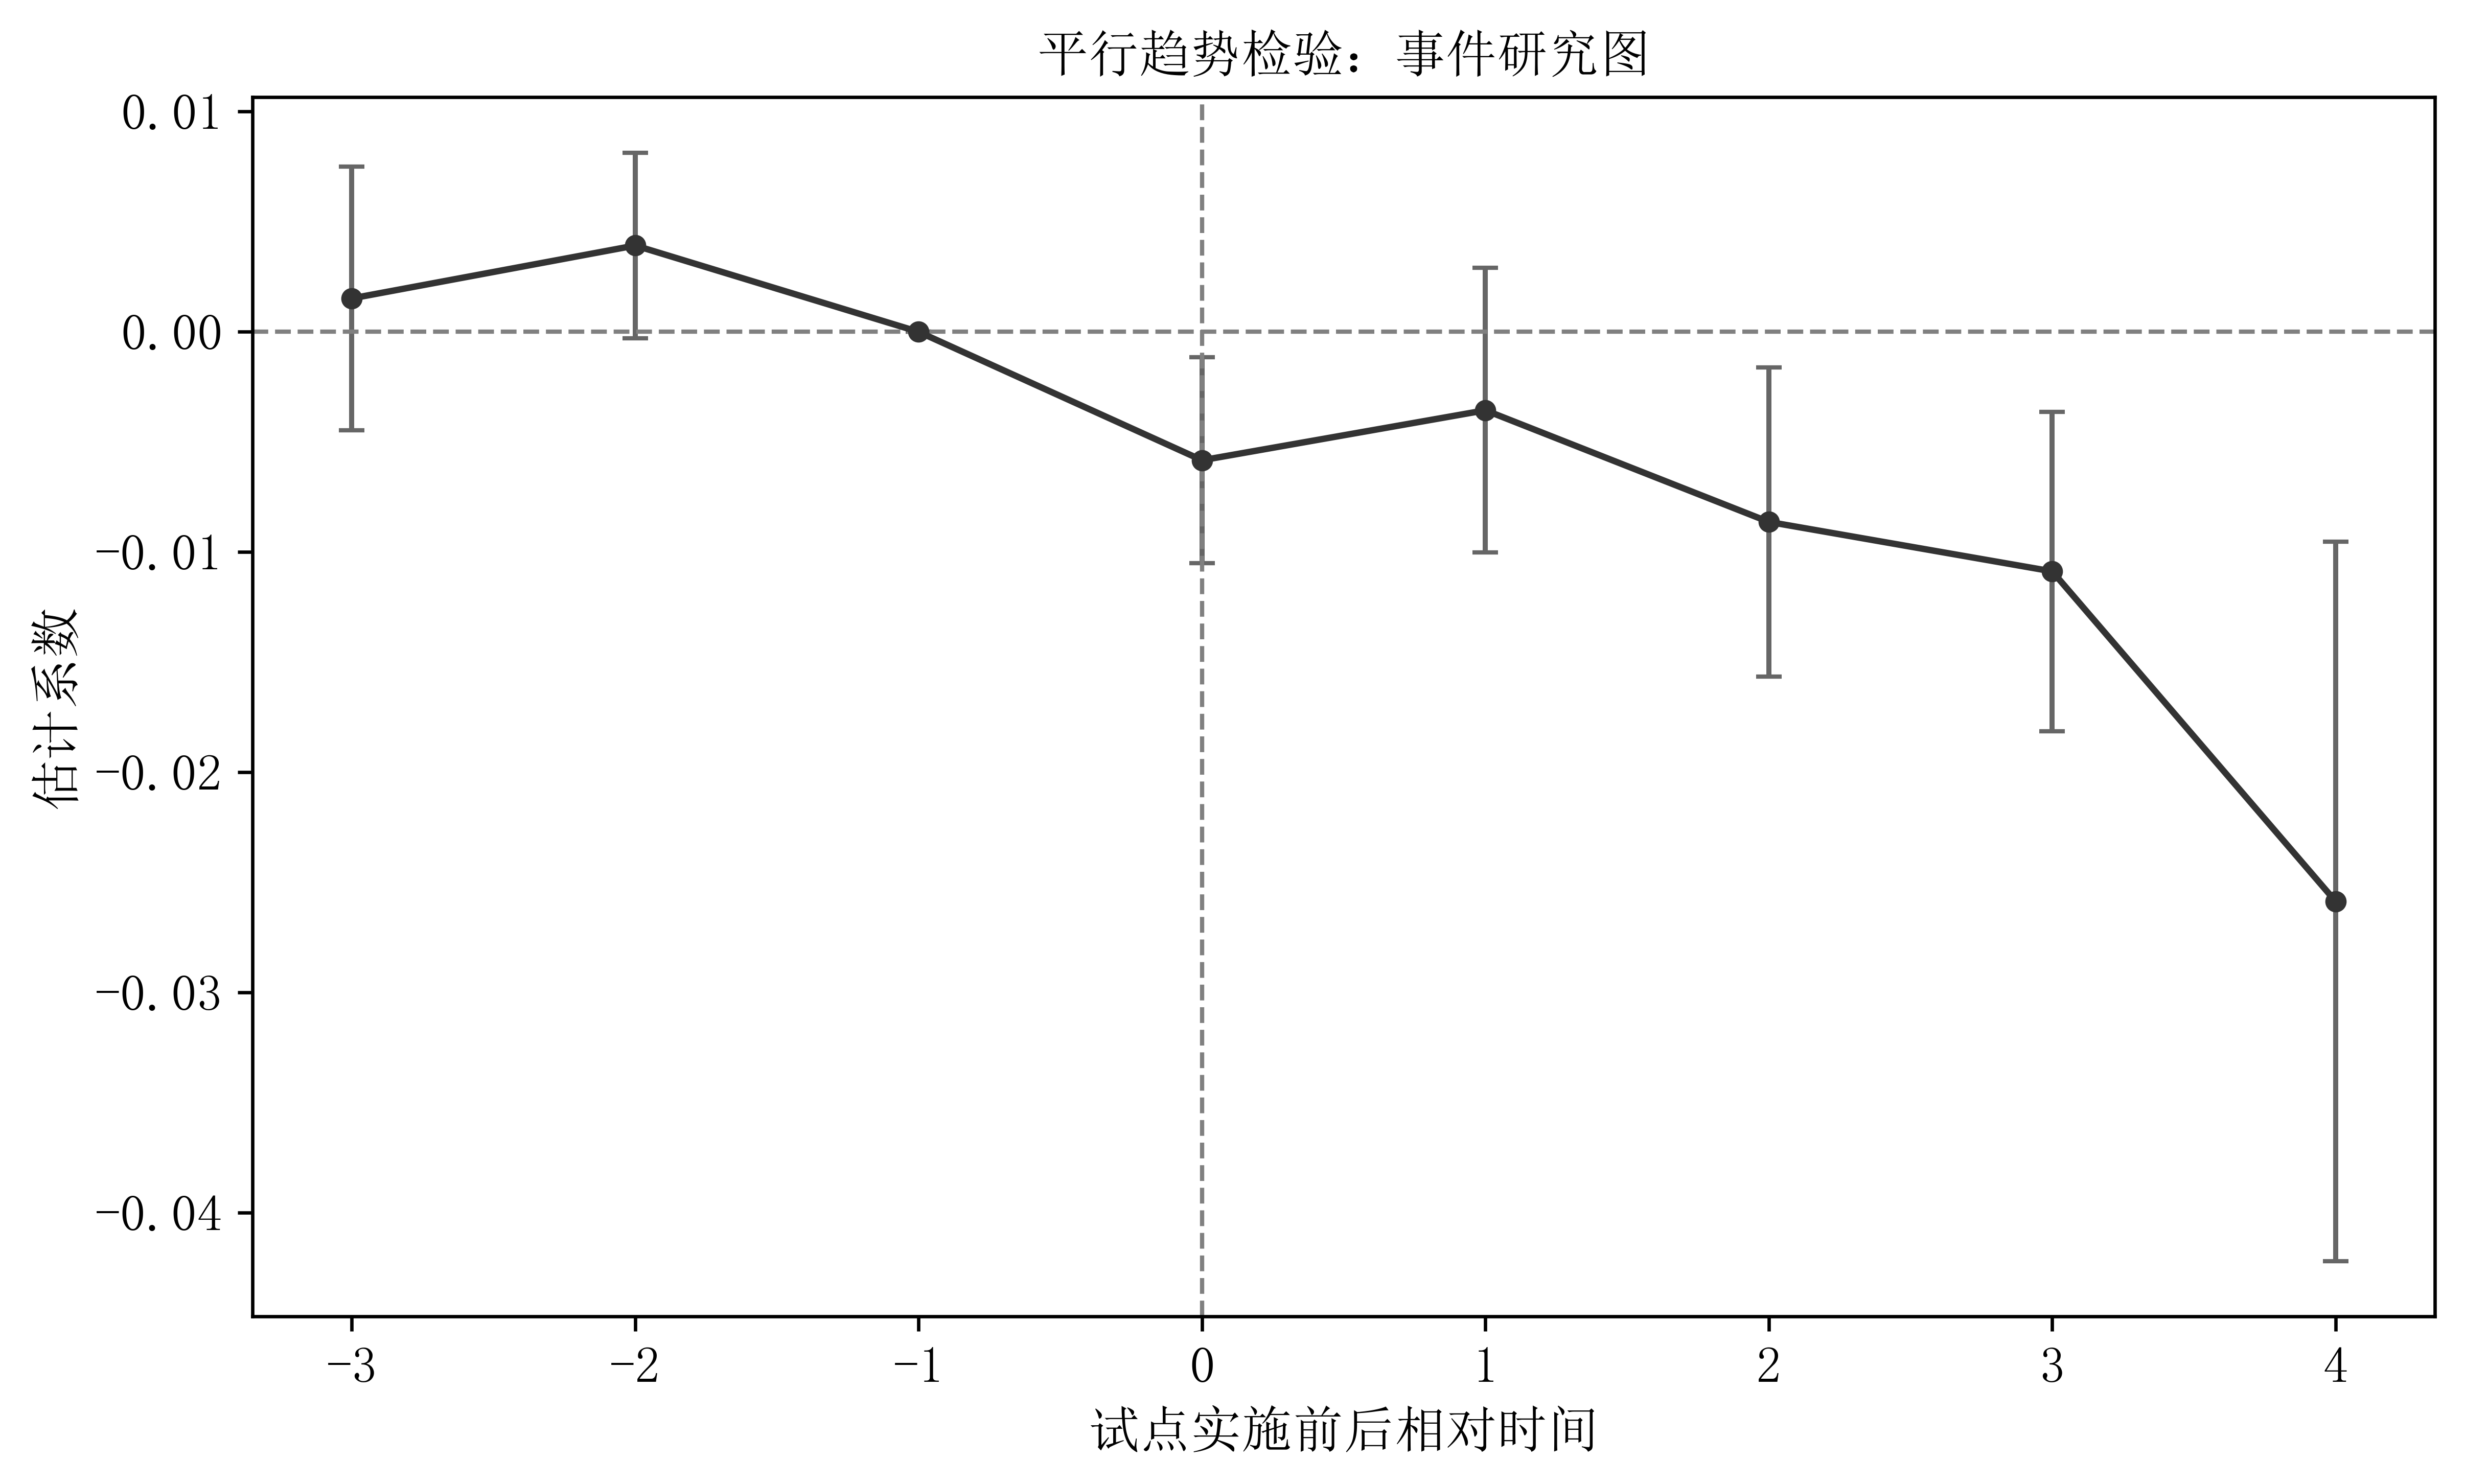
\includegraphics[width=0.82\textwidth]{assets/figures/平行趋势.png}
    \caption{平行趋势检验}
    \label{fig:parallel}
\end{figure}

政策实施前各期估计值总体围绕零波动，且未显著异于0；政策实施后，估计系数逐渐转为负值，并在一年滞后期开始表现出较为明确的负向作用，说明国家低碳城市试点政策对减污降碳压力的缓解作用并非即时完成，而是在政策实施后逐步释放，且政策效果日益显著。这一结果进一步支持了基准回归结论的可信性。

\subsection{安慰剂检验}

为排除不可观测因素、遗漏变量及随机因素对估计结果的影响，本文采用基于虚拟处理组的安慰剂检验。结果显示，真实政策系数 $-0.0152^{***}$ 明显偏离虚拟系数分布，说明随机生成的虚拟政策冲击难以复现真实政策效应，基准回归结论具有较强稳健性。

\begin{figure}[H]
    \centering
    \includegraphics[width=0.78\textwidth]{assets/figures/安慰剂.png}
    \caption{安慰剂检验}
    \label{fig:placebo}
\end{figure}

\section{稳健性检验}

\subsection{双侧缩尾处理}

考虑到城市面板数据中可能存在异常值对模型估计结果产生干扰，本文对被解释变量和控制变量进行 5\% 双侧缩尾处理，并在缩尾后的样本上重新估计基准 DID 模型。结果显示，低碳城市试点政策变量的估计系数为 $-0.0071$，且在 1\% 统计水平上显著，说明在进行双侧缩尾处理后，低碳城市试点政策仍能够显著降低减污降碳压力指数，基准结果较为稳健。

\subsection{时间趋势控制}

多期 DID 模型的有效识别依赖于处理组与控制组在政策实施前具有相似的变化趋势。然而，不同城市在经济发展水平、产业结构、资源禀赋和环境治理基础等方面存在差异，这些基础条件可能导致城市减污降碳压力指数呈现不同的变化趋势。为进一步控制不同城市基础条件可能带来的差异化时间趋势，本文在基准模型中加入控制变量与线性时间趋势的交互项。结果显示，加入时间趋势控制后，低碳城市试点政策变量的估计系数为 $-0.0074$，且在5\%统计水平上显著，表明在进一步控制城市特征所带来的趋势性影响后，低碳城市试点政策仍具有显著的减污降碳作用。

\subsection{PSM-DID}

低碳城市试点政策的实施并非完全随机，试点城市与非试点城市在经济发展水平、产业基础和环境治理能力等方面可能存在系统性差异，从而导致样本选择偏误。因此本文进一步采用 PSM-DID 方法进行稳健性检验。具体而言，本文基于政策实施前控制变量的均值和变化趋势估计倾向得分，并采用近邻匹配方法为试点城市匹配可比的非试点城市。图~\ref{fig:psm_balance}显示，匹配后多数协变量的标准化偏差明显向0靠近，说明匹配后处理组与控制组的协变量平衡性得到改善。在此基础上，本文进一步基于匹配样本重新估计 DID 模型。结果显示，PSM-DID 估计中政策变量系数为 $-0.0087$，且在5\%统计水平上显著，说明在缓解样本选择偏误后，低碳城市试点政策对减污降碳压力指数的减缓作用仍然成立。

\begin{figure}[H]
    \centering
    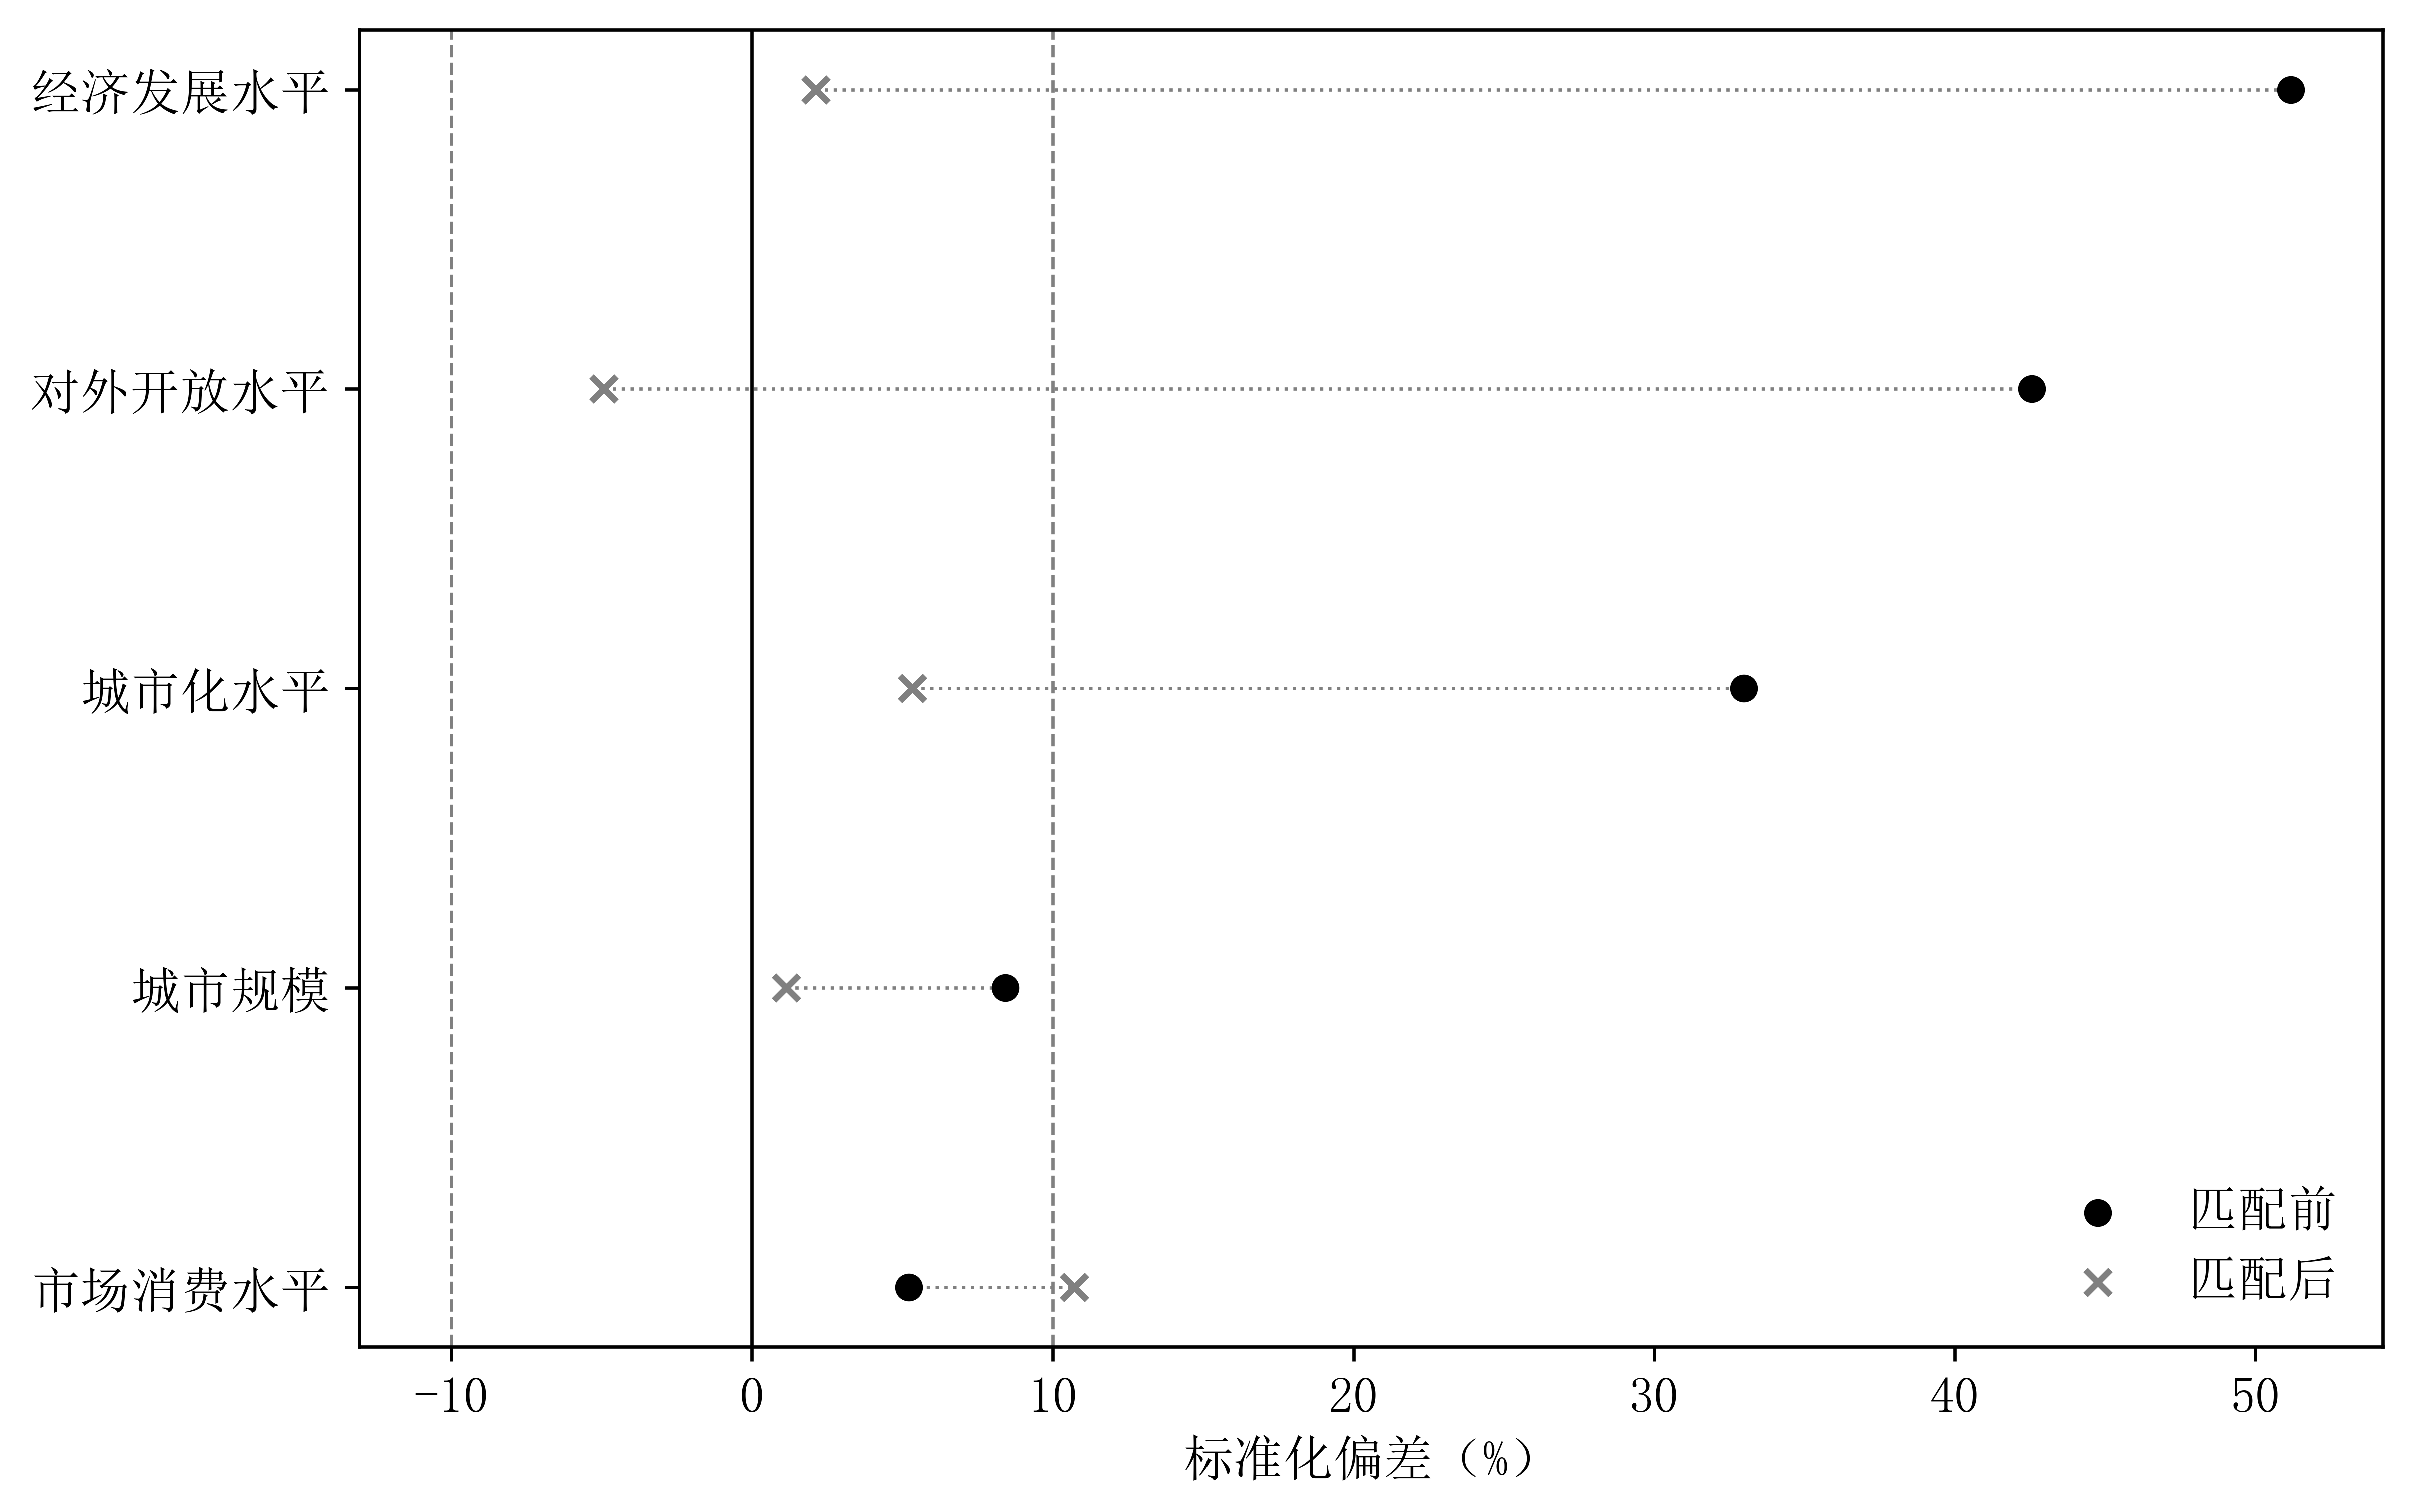
\includegraphics[width=0.82\textwidth]{assets/figures/PSM-DID.png}
    \caption{PSM-DID匹配前后协变量平衡性检验}
    \label{fig:psm_balance}
\end{figure}

\subsection{面板 Tobit}

为检验模型设定变化是否影响本文结论，本文进一步采用 Tobit 模型进行稳健性检验。表~\ref{tab:robust}结果显示，在 Tobit 模型下，低碳城市试点政策变量的估计系数为 $-0.0152^{***}$，且在1\%统计水平上显著。该结果与基准回归的系数方向和显著性保持一致，说明在考虑因变量受限特征后，本文核心结论依然稳健。

\begin{table}[H]
    \centering
    \caption{稳健性检验}
    \label{tab:robust}
    \renewcommand{\arraystretch}{1.2}
    \begin{threeparttable}
    \tablefont
    \setlength{\tabcolsep}{2pt}
    \begin{tabularx}{\textwidth}{C{2.7cm}C{3.0cm}C{3.0cm}C{2.2cm}C{2.5cm}}
        \toprule
        变量符号 & 双侧缩尾处理 & 时间趋势控制 & PSM-DID & 面板 Tobit \\
        \midrule
        DID & -0.0071*** & -0.0074** & -0.0087** & -0.0152*** \\
         & (0.0025) & (0.0035) & (0.0041) & (0.0016) \\
        控制变量 & 是 & 是 & 是 & 是 \\
        城市固定效应 & 是 & 是 & 是 & 是 \\
        年份固定效应 & 是 & 是 & 是 & 是 \\
        样本量 N & 4432 & 4432 & 2448 & 4432 \\
        调整后$R^2$ & 0.9466 & 0.9435 & 0.9346 & -- \\
        \bottomrule
    \end{tabularx}
    \begin{tablenotes}[flushleft]
        \tablenotefont
        \item 注：Tobit 模型采用极大似然估计，调整后 R$^2$ 主要适用于 OLS 回归，故本文未报告 Tobit 模型的调整后 R$^2$。
    \end{tablenotes}
    \end{threeparttable}
\end{table}

\section{基于可解释机器学习的异质性分析}

\subsection{模型对比与选择}

表~\ref{tab:ml_perf}报告了随机森林和 XGBoost 模型的性能。从拟合优度和误差指标看，随机森林在测试集上具有更高的 $R^2$ 以及更低的 RMSE 和 MAE，整体模型性能优于 XGBoost。因此，本文选取随机森林作为后续 TreeSHAP 解释的主模型。

\begin{table}[H]
    \centering
    \caption{模型性能}
    \label{tab:ml_perf}
    \begin{threeparttable}
    \tablefont
    \renewcommand{\arraystretch}{1.2}
    \setlength{\tabcolsep}{2pt}
    \begin{tabularx}{\textwidth}{C{2.6cm}*{4}{>{\centering\arraybackslash}X}}
        \toprule
        模型 & 训练集$R^2$ & 测试集$R^2$ & 测试集RMSE & 测试集MAE \\
        \midrule
        随机森林 & 0.9800 & 0.8604 & 0.0330 & 0.0235 \\
        XGBoost & 0.9061 & 0.8151 & 0.0379 & 0.0289 \\
        \multicolumn{5}{c}{TreeSHAP解释主模型：随机森林} \\
        \bottomrule
    \end{tabularx}
    \begin{tablenotes}[flushleft]
        \tablenotefont
        \item 注：RMSE与MAE越小、$R^2$越高，表明模型样本外性能越好。
    \end{tablenotes}
    \end{threeparttable}
\end{table}

\subsection{特征重要性}

图~\ref{fig:model_feature_importance}显示，城市规模和经济发展水平均位居前列，城市化水平和市场消费水平也具有一定贡献，而对外开放水平和低碳城市试点变量的重要性相对较低。这说明减污降碳压力差异不仅取决于试点政策，也受城市发展基础影响；XGBoost 和 Random Forest 两个模型结果的一致性增强了后续 TreeSHAP 解释的可信度。

\begin{figure}[H]
    \centering
    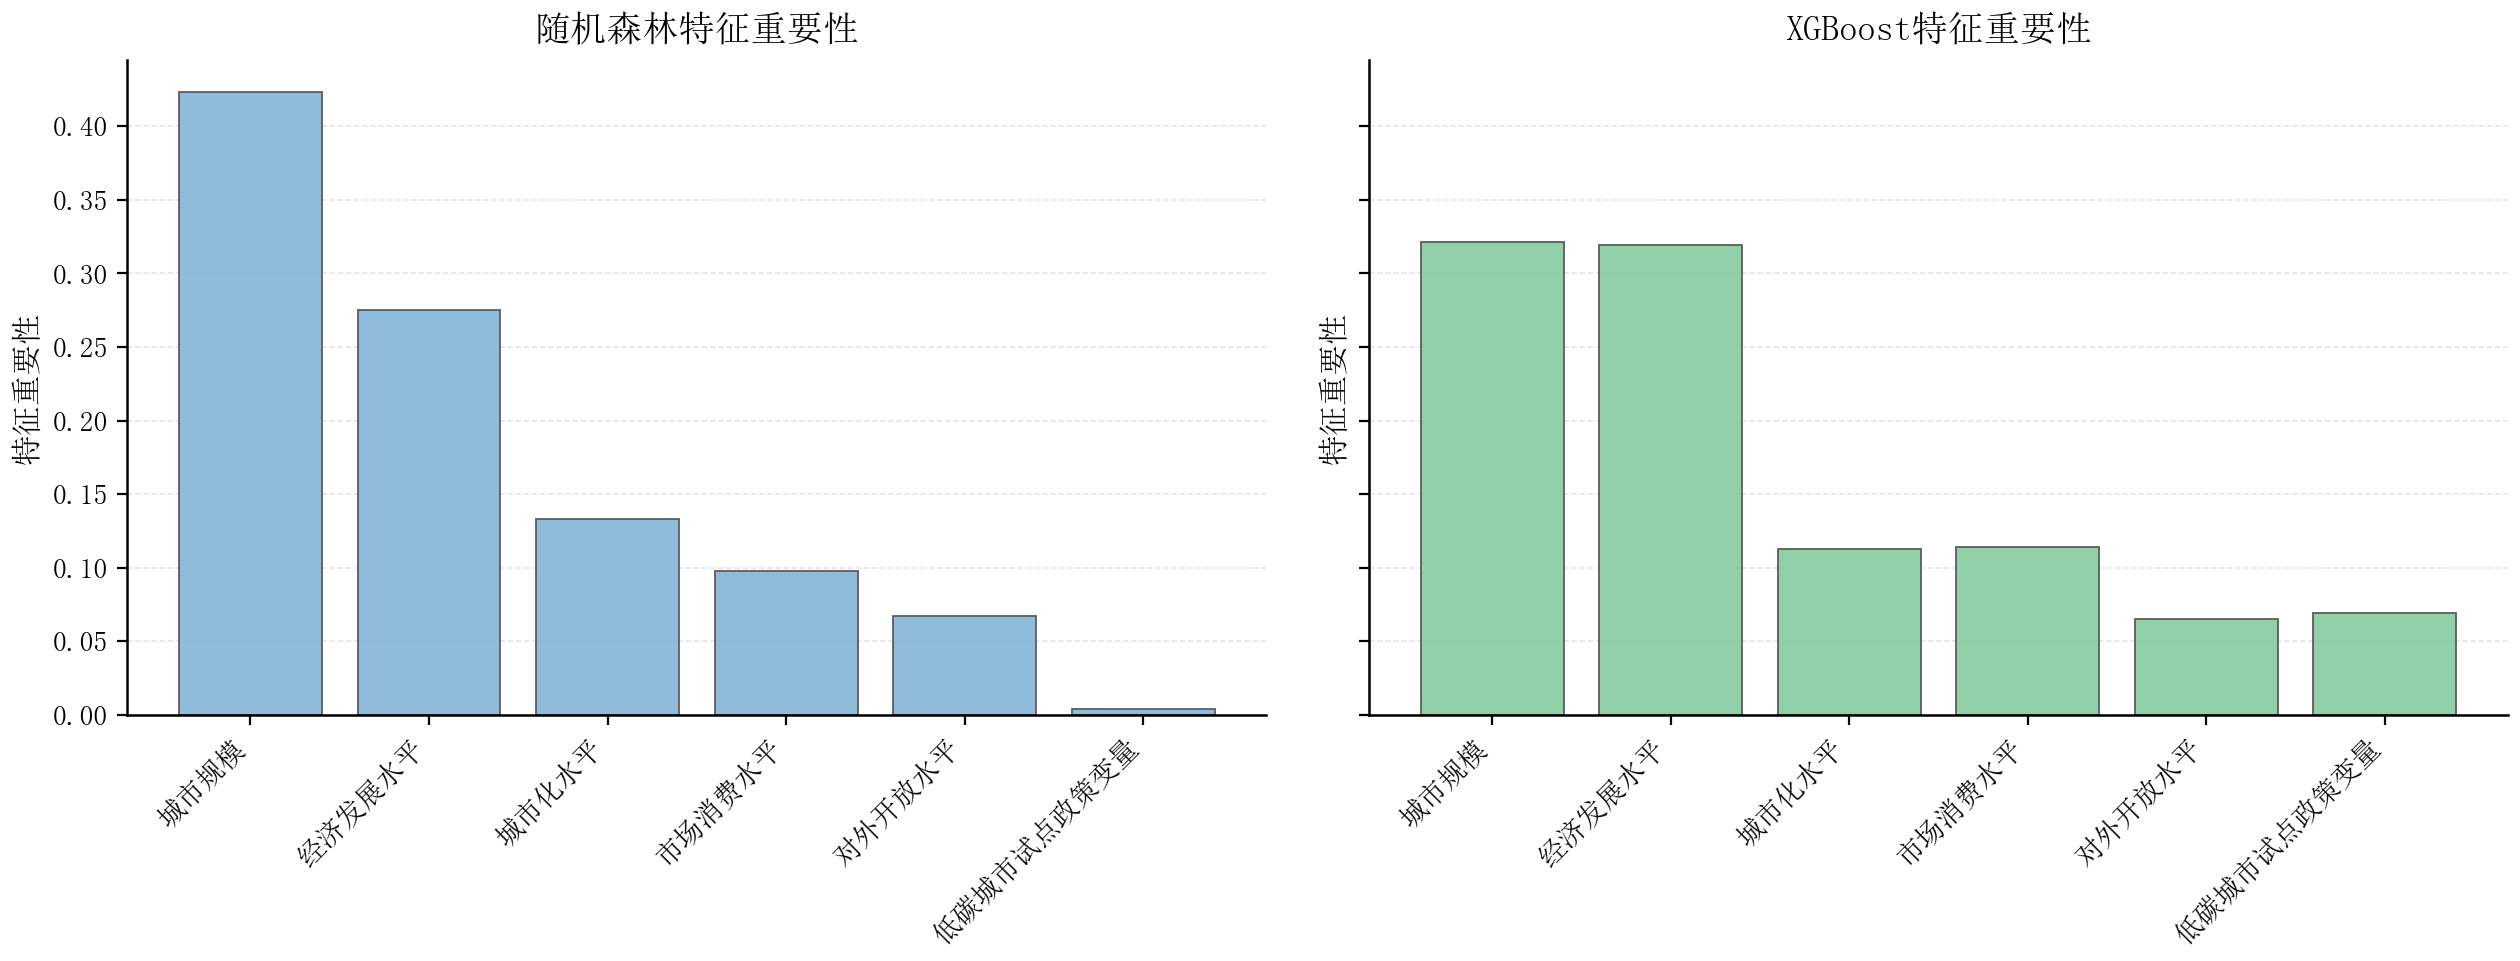
\includegraphics[width=0.96\textwidth]{assets/figures/double_model_feature_importance.png}
    \caption{随机森林与 XGBoost 特征重要性}
    \label{fig:model_feature_importance}
\end{figure}

\subsection{SHAP 特征重要性}

图8展示了随机森林模型的 TreeSHAP 解释结果，其中图8（a）为 SHAP 摘要图，图8（b）为 SHAP 交互图。本文主要依据摘要图分析各变量对模型输出的贡献方向。结果显示，城市规模和经济发展水平是主要影响变量，其 SHAP 值主要分布区间分别为[$-0.0808$,0.0611]和[$-0.0542$,0.0569]；二者高值样本中分别有98.4\%和99.3\%位于 SHAP 正值区域，说明人口规模较大、经济活动强度较高的城市更容易面临较高减污降碳压力。

进一步看，城市化水平的 SHAP 值主要分布在[$-0.0215$,0.0195]，其高值样本中98.4\%位于 SHAP 正值区域，表明较高城市化水平可能通过人口集聚、建设活动和资源消耗增加减污降碳压力；市场消费水平的 SHAP 值主要分布在[$-0.0157$,0.0236]，其高值样本中96.3\%位于 SHAP 负值区域，说明消费水平较高、服务业基础较强的城市减污降碳压力相对较低。图8（b）进一步显示，减污降碳压力受到多维城市基础条件的共同作用。

\begin{figure}[H]
    \centering
    % 注：若最终提交版本要求图中文字严格区分字体，需重新导出该图，确保中文为宋体、英文和数字为 Times New Roman。
    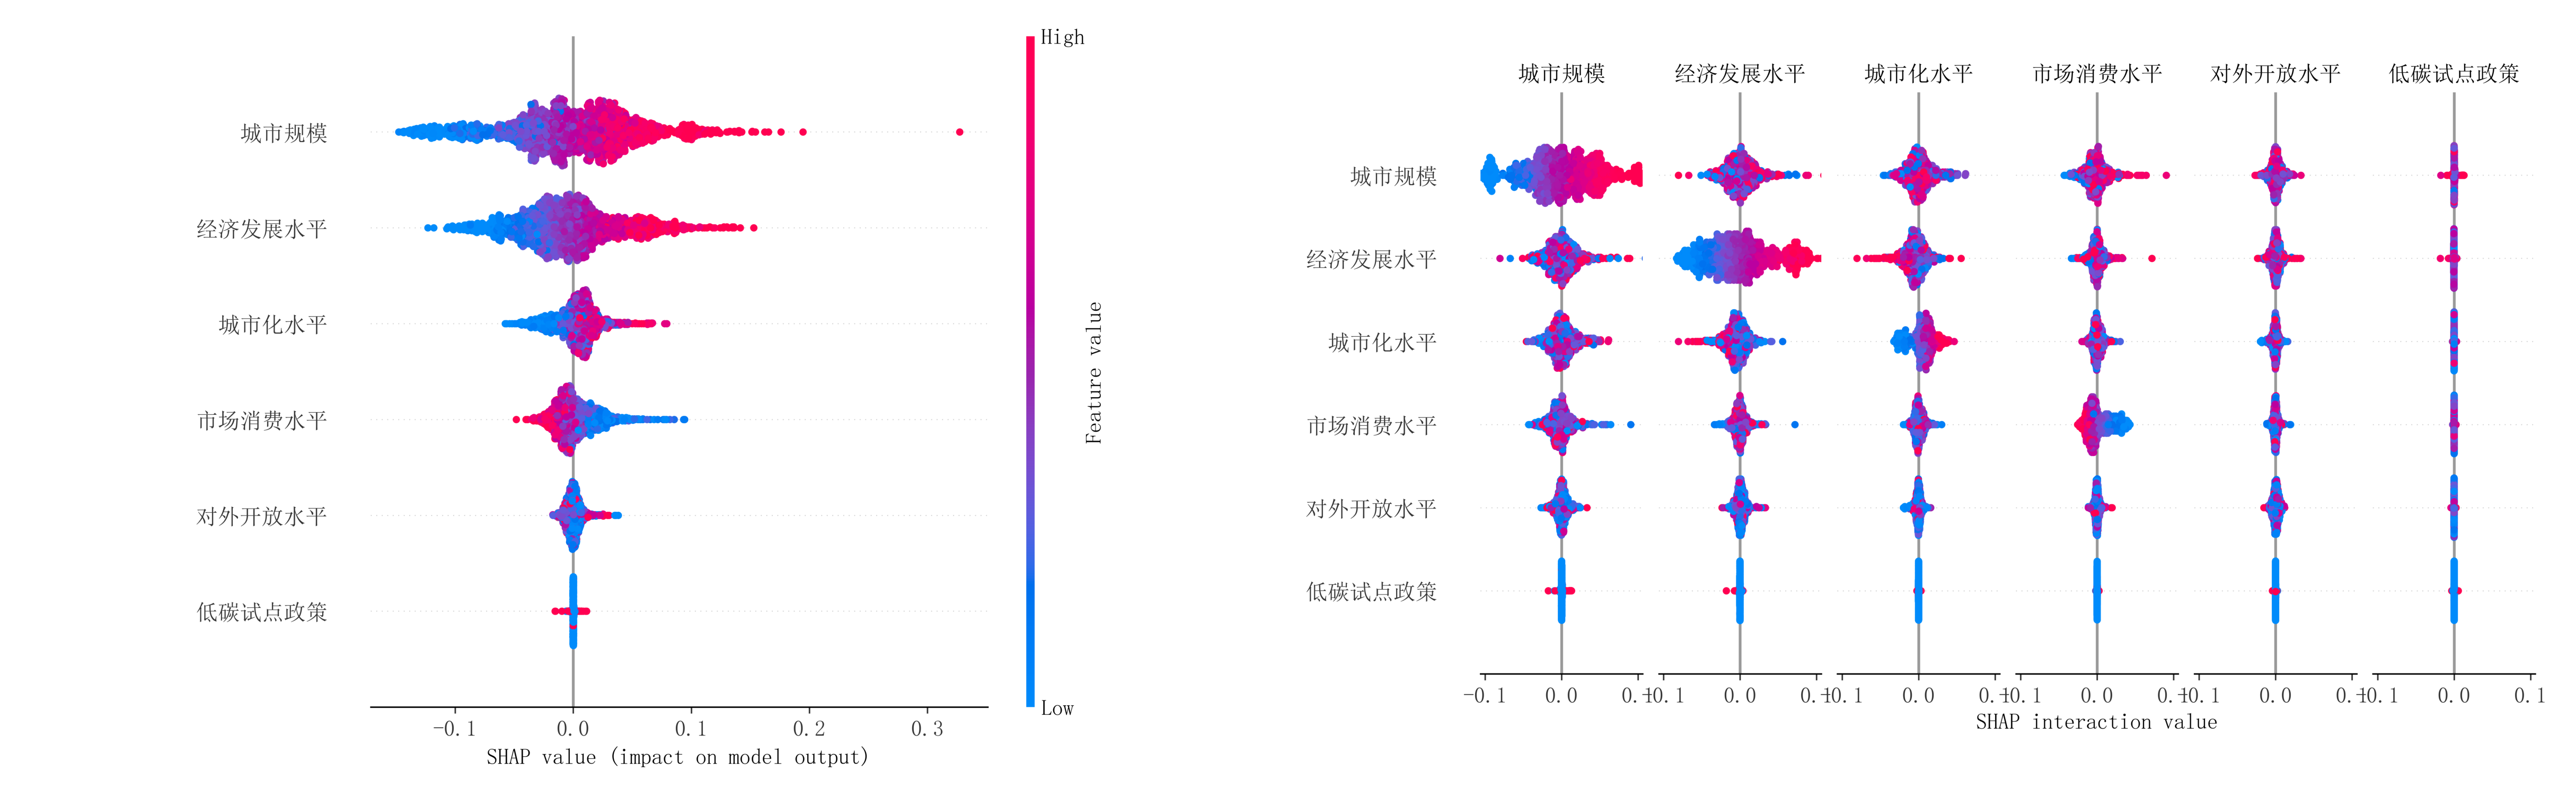
\includegraphics[width=\textwidth]{assets/figures/shap_feature_importance.png}
    \caption*{（a）SHAP 摘要图\hspace{4em}（b）SHAP 交互图}
    \caption{SHAP 特征重要性}
    \label{fig:shap_summary}
\end{figure}

\section{进一步讨论}

\subsection{绿色创新中介效应}

表~\ref{tab:mediation}报告了绿色创新的中介效应检验结果。第（1）列以绿色创新为因变量，结果显示低碳城市试点政策变量系数为1.3727，且在1\%统计水平上显著，说明试点政策显著提升了城市绿色创新水平。第（2）列报告政策对减污降碳压力指数的总效应，政策变量系数为 $-0.0152^{***}$。第（3）列进一步加入绿色创新变量后，政策变量系数收缩至 $-0.0090$，且仍在1\%统计水平上显著；绿色创新变量系数为 $-0.0045$，并在5\%统计水平上显著。上述结果表明，绿色创新在低碳城市试点政策降低减污降碳压力的过程中发挥部分中介效应，假设H2得到验证。

\begin{table}[H]
    \centering
    \caption{中介效应}
    \label{tab:mediation}
    \begin{threeparttable}
    \renewcommand{\arraystretch}{1.2}
    \tablefont
    \begin{tabularx}{\textwidth}{C{3.2cm}C{3.0cm}C{3.1cm}C{3.4cm}}
        \toprule
        \multirow{2}{*}{\raisebox{-0.3ex}{\makebox[3.2cm][c]{变量符号}}} & (1) & (2) & (3) \\
          & greeninnov & Pressure & Pressure \\
        \midrule
        DID & 1.3727*** & -0.0152*** & -0.0090*** \\
          & (0.3627) & (0.0040) & (0.0034) \\
        greeninnov &  &  & -0.0045** \\
          &  &  & (0.0019) \\
        控制变量 & 是 & 是 & 是 \\
        城市固定效应 & 是 & 是 & 是 \\
        年份固定效应 & 是 & 是 & 是 \\
        样本量 N & 4432 & 4432 & 4432 \\
        调整后$R^2$ & 0.6950 & 0.9380 & 0.9410 \\
        Bootstrap间接效应 & \multicolumn{3}{c}{-0.0062} \\
        95\% CI & \multicolumn{3}{c}{[-0.0113,\,-0.0029]} \\
        间接效应占比 & \multicolumn{3}{c}{41.0\%} \\
        \bottomrule
    \end{tabularx}
    \begin{tablenotes}[flushleft]
        \tablenotefont
        \item 注：绿色创新变量已换算为原始绿色创新/1000，绿色创新系数表示绿色创新每增加 1000 单位时对减污降碳压力指数的影响。
    \end{tablenotes}
    \end{threeparttable}
\end{table}

Bootstrap 间接效应检验的 95\% 置信区间为 [-0.0113，-0.0029]，不包含0，说明绿色创新中介效应显著存在；间接效应占比为41.0\%，表明低碳城市试点政策有相当一部分减污降碳作用是通过提升绿色创新实现的。基于此，政府应通过财政补贴、绿色信贷、研发平台建设和知识产权保护等方式，加大对绿色技术研发和成果转化的支持力度，从而强化低碳城市试点政策的长期传导效果。

\subsection{产业结构调节效应}

表~\ref{tab:moderation}报告了产业结构合理化变量的调节效应检验结果。列（3）中，产业结构合理化变量与政策变量的交互项系数为0.0418，并在 1\% 统计水平上显著。这表明产业结构合理化变量在低碳城市试点政策降低减污降碳压力的过程中发挥负向调节效应，假设 H3 得到验证。换言之，结合 TL 指标方向来看，交互项显著为正说明产业结构偏离均衡状态会削弱低碳城市试点政策降低减污降碳压力的作用。这是因为产业结构偏离会加剧要素错配，使资源更多集中于高耗能、高排放部门，从而削弱政策的减污降碳效果。

\begin{table}[H]
    \centering
    \caption{调节效应}
    \label{tab:moderation}
    \renewcommand{\arraystretch}{1.2}
    \begin{threeparttable}
    \tablefont
    \setlength{\tabcolsep}{1.5pt}
    \begin{tabularx}{\textwidth}{C{4.6cm}C{3.0cm}C{3.0cm}C{3.0cm}}
        \toprule
        变量符号 & (1) & (2) & (3) \\
        \midrule
        DID $\times$ TL & -0.0914 & 0.0444*** & 0.0418*** \\
          & (0.0664) & (0.0137) & (0.0123) \\
        TL & -0.1104*** & -0.0146** & -0.0086 \\
          & (0.0192) & (0.0072) & (0.0073) \\
        DID & 0.0615*** & -0.0246*** & -0.0245*** \\
          & (0.0175) & (0.0051) & (0.0049) \\
        控制变量 & 否 & 否 & 是 \\
        城市固定效应 & 否 & 是 & 是 \\
        年份固定效应 & 否 & 是 & 是 \\
        样本量 N & 4160 & 4160 & 4160 \\
        调整后$R^2$ & 0.1100 & 0.9330 & 0.9360 \\
        \bottomrule
    \end{tabularx}
    \begin{tablenotes}[flushleft]
        \tablenotefont
        \item 注：括号内为按城市层级聚类的稳健标准误；*、**、***分别表示在10\%、5\%、1\%水平上显著。
    \end{tablenotes}
    \end{threeparttable}
\end{table}

\section{结论与建议}

\subsection{研究结论}

本文基于2006—2021年中国277个城市面板数据，构建减污降碳压力指数，并采用多期 DID 模型评估低碳城市试点政策的实施效果。基准回归结果表明，低碳城市试点政策能够显著降低城市减污降碳压力，影响系数为 $-0.0152^{***}$。平行趋势检验支持识别前提，安慰剂检验、双侧缩尾处理、时间趋势控制、PSM-DID和面板 Tobit 结果均验证了结论稳健性。

机制分析表明，绿色创新在低碳城市试点政策降低减污降碳压力的过程中发挥部分中介效应；产业结构合理化变量发挥负向调节效应，产业结构偏离均衡状态越明显，低碳城市试点政策缓解减污降碳压力的作用越弱。

可解释机器学习进一步揭示了城市异质性。TreeSHAP 结果显示，城市规模、经济发展水平、城市化水平和市场消费水平是解释城市减污降碳压力差异的重要因素。

\subsection{政策建议}

第一，完善低碳城市试点政策设计，统筹推进降碳、减污、节能和产业转型。地方政府应建立动态评估机制，根据城市减污降碳压力变化及时调整政策重点。

第二，强化绿色创新支持，提升低碳试点政策的传导效果。政府可通过财政补贴、绿色信贷和研发平台建设，引导企业加大绿色技术研发和成果转化投入。

第三，结合城市产业结构和发展基础差异，推进精准化、差异化治理。高耗能、高排放产业占比较高的城市应侧重技术改造和产业优化，基础较好的城市应强化绿色技术扩散和低碳转型带动作用。

% ==================== 参考文献 ====================
\newpage
\begin{thebibliography}{99}
\bodyfont

\bibitem{ref:cheng2025}
成喜玲，胡照远. 低碳城市试点政策的污碳协同减排效应研究[J]. 国土资源科技管理，2025，42(4)：108-118.

\bibitem{ref:gan2011}
干春晖，郑若谷，余典范. 中国产业结构变迁对经济增长和波动的影响[J]. 经济研究，2011，46(5)：4-16，31.

\bibitem{ref:ndrc2010}
国家发展和改革委员会. 关于开展低碳省区和低碳城市试点工作的通知[Z]. 2010.

\bibitem{ref:ndrc2012}
国家发展和改革委员会. 关于开展第二批国家低碳省区和低碳城市试点工作的通知[Z]. 2012.

\bibitem{ref:ndrc2017}
国家发展和改革委员会. 关于开展第三批国家低碳城市试点工作的通知[Z]. 2017.

\bibitem{ref:hao2025}
郝浩宇，黄旭辉，张宁. 网络基础设施建设能提升城市全要素碳生产率吗？[J]. 中国人口·资源与环境，2025，35(3)：46-56.

\bibitem{ref:huang2023}
黄寰，何广，肖义. 低碳城市试点政策的碳减排效应[J]. 资源科学，2023，45(5)：1044-1058.

\bibitem{ref:liu2024}
刘明亮，尹晶晶，李华清，林剑艺. 减污降碳协同效率时空演化特征及驱动机制研究：基于中国三大城市群[J]. 生态经济，2024，40(7)：174-183.

\bibitem{ref:luo2024}
罗良文，雷朱家华. 中国碳市场政策的减污降碳协同效应[J]. 资源科学，2024，46(1)：53-68.

\bibitem{ref:plan2022}
生态环境部等. 减污降碳协同增效实施方案[Z]. 2022.

\bibitem{ref:sun2025}
孙慧，张学峰，夏学超，杨泽东，祝树森. 用能权交易制度与低碳城市双试点协同的降碳减污效应[J]. 中国人口·资源与环境，2025，35(3)：25-35，11.

\bibitem{ref:wen2004}
温忠麟，张雷，侯杰泰，刘红云. 中介效应检验程序及其应用[J]. 心理学报，2004，36(5)：614-620.

\bibitem{ref:xing2024}
邢华，李向阳. 减污降碳：低碳城市试点的协同效应[J]. 干旱区资源与环境，2024，38(5)：10-19.

\bibitem{ref:zhang2026}
张梦雨，马晓钰. 新基建能否实现减污降碳协同效应: 来自特高压输电工程的证据[J]. 经济经纬，2026，43(1)：17-31.

\bibitem{ref:zhangxuechun2024}
张雪纯，曹霞，宋林芷. 碳排放交易制度的减污降碳效应研究：基于合成控制法的实证分析[J]. 自然资源学报，2024，39(3)：712-730.

\bibitem{ref:abadie2005}
Abadie A. Semiparametric difference-in-differences estimators[J]. The Review of Economic Studies, 2005, 72(1): 1-19.

\bibitem{ref:breiman2001}
Breiman L. Random forests[J]. Machine Learning, 2001, 45(1): 5-32.

\bibitem{ref:chen2016}
Chen T, Guestrin C. XGBoost: A scalable tree boosting system[C]//Proceedings of the 22nd ACM SIGKDD International Conference on Knowledge Discovery and Data Mining. 2016: 785-794.

\bibitem{ref:lundberg2017}
Lundberg S M, Lee S I. A unified approach to interpreting model predictions[C]//Advances in Neural Information Processing Systems. 2017, 30: 4765-4774.

\bibitem{ref:porter1995}
Porter M E, van der Linde C. Toward a new conception of the environment-competitiveness relationship[J]. Journal of Economic Perspectives, 1995, 9(4): 97-118.

\end{thebibliography}

\end{document}
 2.
